
\begin{refsection}
\startcontents[chapters]	
\chapter{Theory of Statistical Distribution}\label{ch:theory-of-statistics}
%\minitoc

\printcontents[chapters]{}{1}{}
\section{General remarks}

\subsection{The goal and task of statistical inference}
\begin{itemize}
	\item Given observations of random variable $X$, the \textbf{ultimate goal} of statistical inference is to infer the distribution of $X$.
	\item Limited observation data usually make direct inference on the distribution of $X$ impractical.
	\item We subjectively \textbf{assume} the distribution of $X$ is given by some parameterized statistical model(e.g. Gaussian, Binomial,Poisson). More commonly, a statistical model is written as a set of distributions for $X$, $\cP=\{P_\theta,\theta\in\Omega\}$, where $\Omega$ is the parameter space containing all possible values of $\theta$. Note that a statistical model is a hypothesis, which might be correct or incorrect.
	\item With the statistical model proposed, we estimate the model parameter $\theta$ from the data. Once estimated, we have a way to describe the distribution of $X$, which finishes the inference task.
\end{itemize}

\subsection{Major components in statistical inference}
\begin{itemize}
	\item There are two major components in statistical inference: \textbf{statistical models} and \textbf{estimating model parameters}.
	\item We usually restrict ourselves to \textbf{ mathematically convenient models}, such as exponential families, such that useful properties of the distribution, such as mean and variance, can be easily derived.  
	\item We design statistic $\delta$, which is a function of random sample $X$, such that $\delta$ is closed to $\theta$ or $g(\theta)$. In this way, we use statistic to relate data $X$ to model parameter $\theta$.
	\begin{itemize}
		\item Not all statistics are equally good. Some are biased: $E\delta_\theta \neq \theta$. Some are more efficient in terms of using information to reduce uncertainty.
		\item We can use mean-square-error(MSE), or more general risk functions to evaluate of a statistic. 
	\end{itemize}
	
\end{itemize}

\section{Common distributions and properties}




\subsection{Bernoulli distribution}
\begin{definition}[Bernoulli distribution]\index{Bernoulli distribution}
	A random variable $Y$ with sample space $\{0,1\}$ is said to have Bernoulli distribution $Ber(\theta)$ with parameter $\theta$ if it has a pmf given as
	$$p(y) = \theta^y(1-\theta)^{1-y}, y\in \{0,1\}.$$
\end{definition}

\begin{lemma}[basic properties]\label{ch:theory-of-statistics:th:Bernoullidistributionproperty}
Let $X$ be a random variable with distribution $Ber(p)$. Then
\begin{itemize}
	\item $M_X(t) = (1 - p + pe^t)$.
	\item $E[X] = p, E[X^2] = p, Var[X^2] = p - p^2 = p(1-p).$
\end{itemize}
\end{lemma}
\begin{proof}
Straight forward.
\end{proof}



\subsection{Normal distribution}\index{normal distribution}\label{ch:theory-of-statistics:sec:normaldistribution}
\begin{definition}\cite[171]{hoggintroduction}[normal distribution]
A random variable $X$ is said to have normal distribution $N(\mu,\sigma^2)$ with parameter $\mu$ and $\sigma$ if its pdf is given as
$$f(x) = \frac{1}{\sqrt{2\pi} \sigma} \exp(-\frac{1}{2}(x-\mu)^2/\sigma^2),-\infty < x <\infty $$
\end{definition}


\begin{lemma}[moment generating function]
Let $X$ be a random variable with normal distribution $N(0,1)$, then the moment generating function is
$$m_X(t) = \exp(\frac{1}{2}t^2).$$
If $Y$ is a random variable with normal distribution $N(\mu,\sigma^2)$, then the moment generating function is
$$m_Y(t) = \exp(\mu t + \frac{1}{2}\sigma^2 t^2).$$
\end{lemma}
\begin{proof}
(1) $m_X(t) = E[e^{tX}] = \int_{-\infty}^{\infty} e^{tx}\frac{1}{\sqrt{2\pi}}e^{-\frac{1}{2}x^2}$
complete the square and get the result.
(2)Let $Y=\sigma X + \mu$ and use \autoref{ch:theory-of-probability:th:additionandscalingtheoremformgf}. Then $m_Y(t) = e^{\mu t}m_X(\sigma t)$	
\end{proof}

\begin{lemma}[Basic properties]\label{ch:theory-of-statistics:th:basicnormalproperties}
Consider $X\sim N(\mu_x,\sigma^2_x), Y\sim N(\mu_y,\sigma^2_y)$.
\begin{itemize}
	\item  If \textbf{$X,Y$ are independent}, then we have
	\begin{itemize}
		\item $$aX + b \sim N(a\mu + b, a^2\sigma_x^2)$$
		\item  $$X+Y \sim N(\mu_x+\mu_y,\sigma_x^2 + \sigma_y^2)$$
		$$aX+bY \sim N(a\mu_x+b\mu_y,a^2\sigma_x^2 + b^2 \sigma_y^2)$$
	\end{itemize}
	\item  If \textbf{$X$ and $Y$ are not independent but jointly normal}, then $X+Z$ will be normal, and
	$$aX + bZ \sim N(a\mu_x+b\mu_y,a^2\sigma_x^2 + b^2\sigma_z^2 + 2abCov(X,Z)).$$
	\item  Assume $X, Y$ are independent. Further let $W = \rho X + \sqrt{1-\rho^2}Y, \rho\in [-1,1]$. Then
	 $W$ is normal, correlated with $X$ and $Y$, and the sum $X+W$ is also normal; that is, 
	 $$W\sim N, aX+bW\sim N.$$
	 \item \textbf{In general, the sum of two dependent normal random variable is not necessarily normal.} See \autoref{ch:theory-of-statistics:th:sumofmultivariatenormalwithjointnormality}.
\end{itemize}
\end{lemma}
\begin{proof}
(1) Directly from the properties of moment generating functions at \autoref{ch:theory-of-probability:th:additionandscalingtheoremformgf}.
(2)The proof of two general jointly normal random variable will be showed in \autoref{ch:theory-of-statistics:th:sumofmultivariatenormalwithjointnormality}.
(3) Note that 
$$(X,W)^T = (X,\rho X + \sqrt{1-\rho^2}Y)^T = \begin{bmatrix}
1 & 0\\
\rho & \sqrt{1-\rho^2}
\end{bmatrix} (X,Y)^T,$$
therefore $(X,W)$ are jointly normal(\autoref{ch:theory-of-statistics:th:affinetransformmultivariatenormal}). Then we use (2).
\end{proof}


\begin{lemma}[moments of standard normal distribution]\label{ch:theory-of-statistics:th:MomentsOfStandardNormalDistribution}
Let $X\sim N(0,1)$, then
$$E[X] = 0, E[X^2]=1, E[X^3] = 0, E[X^4] = 3$$
Moreover, all odd moments are 0.
\end{lemma}
\begin{proof}
The mgf is $m(t)=e^{t^2/2}$, then
$$m'(t) = te^{t^2/2}$$
$$m''(t) = e^{t^2/2} + t^2e^{t^2/2}$$
$$\dots$$
For all odd moments
$$\int x^{2k+1}f(x)dx$$
has integrand as odd function. 
\end{proof}

\begin{corollary}[moments of normal distribution]
Let $X\sim N(0,\sigma^2)$, then
$$E[X] = 0, E[X^2]=\sigma^2, E[X^3] = 0, E[X^4] = 3\sigma^4$$
Moreover, all odd moments are 0.
\end{corollary}
\begin{proof}
	The mgf is $m(t)=e^{\sigma^2t^2/2}$, then
	$$m'(t) = \sigma^2te^{\sigma^2t^2/2}$$
	$$m''(t) = \sigma^2e^{\sigma^2t^2/2} + \sigma^4t^2e^{t^2/2}$$
	$$\dots$$
	For all odd moments
	$$\int x^{2k+1}f(x)dx$$
	has integrand as odd function. 
\end{proof}

\subsection{Half-normal distribution}
\begin{definition}[half-normal distribution] Let $X$ follow an ordinary normal distribution $N(0, \sigma^2)$. Then $Y=\abs{X}$ follows a half-normal distribution with parameter $\sigma$. It has probability density function
	$$f_Y(y;\sigma) = \frac{\sqrt{2}}{\sigma\sqrt{\pi}}\exp(-\frac{y^2}{2\sigma^2}).$$	
\end{definition}

\begin{lemma}[basic properties of half normal distribution]
Let $Y$ follow a half-normal distribution with parameter $\sigma$. Then\begin{itemize}
	\item $E[Y] = \frac{\sigma\sqrt{2}}{\sqrt{\pi}}$.
	\item $Var[Y] = \sigma^2(1- \frac{2}{\pi})$
\end{itemize}
\end{lemma}

\subsection{Laplace distribution}
\begin{definition}[Laplace distribution]
A random variable $X$ has a Laplace distribution, denoted by $Lap(\mu,b)$, if its probability density function is
$$f(x|\mu,b) = \frac{1}{2b}\exp(-\frac{\abs{x-\mu}}{b}) = \begin{cases*}
\frac{1}{2b}\exp(-\frac{\mu-x}{b}), if~x<\mu \\
\frac{1}{2b}\exp(-\frac{x-\mu}{b}), if~x\geq \mu \\
\end{cases*}.$$	
\end{definition}

\begin{lemma}[properties of Laplace distribution]\label{ch:theory-of-statistics:th:PropertiesOfLaplaceDistribution}
Let $X$ be a random variable with Laplace distribution with parameter $\mu,b$. 
It follows that
\begin{itemize}
	\item The mean and the median are $\mu$.
	\item The variance is $2b^2$.
	\item The cdf is given by
	$$F(x) = \int_{-\infty}^{x} f(u) du =\begin{cases*}
	\frac{1}{2}\exp(-\frac{\mu-x}{b}), if~x<\mu \\
	1-\frac{1}{2}\exp(-\frac{x-\mu}{b}), if~x\geq \mu \\
	\end{cases*} = \frac{1}{2} + \frac{1}{2}sgn(x-\mu)(1 - \exp(-\frac{\abs{x-\mu}}{b})).$$
	\item The inverse cdf is given by
	$$F^{-1}(p) = \mu - b\cdot sgn(p-0.5)\ln(1-2\abs{p-0.5}).$$
\end{itemize}	
\end{lemma}

\subsection{Multivariant Gaussian distribution}
\subsubsection{Basic definitions}
\begin{definition}\cite[180]{hoggintroduction}\index{multivariate Gaussian/normal distribution}
	\cite[40]{chirikjian2011stochastic1}The multivariate Gaussian/normal distribution on $\R^n$ is defined as
	$$\rho(x;\mu,\Sigma) = \frac{1}{(2\pi)^{n/2}\abs{det \Sigma}^{1/2}}\exp(-\frac{1}{2}(x-\mu)^T\Sigma^{-1}(x-\mu))$$
	with mean $\mu \in \R^n$ and covariance matrix $\Sigma$.
	A random vector is said be multivariate Gaussian/normal if it's pdf is multivariate Gaussian/normal distribution.
\end{definition}

\begin{lemma}[alternative definition via mgf]\label{ch:theory-of-statistics:th:multivariateGaussianMGF}\cite[181]{hoggintroduction}
An $n$-dimensional random vector $X$ has a multivariate normal distribution with mean vector $\mu$ and covariance matrix $\Sigma$ if its mgf is
$$M_X(t) = \triangleq E[\exp(t^TX)] = \exp(t^T\mu + \frac{1}{2}t^T\Sigma t)$$
for all $t\in \R^n$.
\end{lemma}
\begin{proof}
\begin{align*}
M_X(t) &= E[\exp(t^TX)] \\
& = \exp(E[t^TX] + \frac{1}{2}Var[t^TX]) \\
& = \exp(t^T\mu + \frac{1}{2}t^T\Sigma t) \\
\end{align*}
where we use the fact that $t^TX\sim N(t^T \mu, t^T\Sigma t)$ from \autoref{ch:theory-of-statistics:th:affinetransformmultivariatenormal}.
\end{proof}

\begin{remark}[implication]
Given a random vector $X$, if we want to check whether $X$ is a multivariate Gaussian, we can check its mgf. If its mgf is the exponential of a linear form plus a quadratic form, then it is multivariate Gaussian. 	
\end{remark}

\begin{lemma}[alternative definition via linear combination]\label{ch:theory-of-statistics:th:MultivariateGaussianDefinitionViaLinearCombination}
A vector $X = (X_1,X_2,...,X_n)^T$ is a multivariate Gaussian distribution if every linear combination 
$$S = a^T X, a\in \R^n$$
has a normal distribution.
\end{lemma}
\begin{proof}
Because $a^TX$ is normal, then it has characteristic function 
$$E[\exp(i ta^TX)] = \exp(ita^T\mu_X - \frac{1}{2}t^2(a)^T\Sigma_X a).$$
Since $a$ is arbitrary, we can say for any $t'\in \R^n$, we have
$$E[\exp(i t'X)] = \exp(i[t']^T\mu_X - \frac{1}{2}[t']^T\Sigma_X t).$$
That is, $X$ is multivariate Gaussian. 
\end{proof}


\begin{example}[bivariate Gaussian distribution]\hfill
Let $f(x,y)$ be the density of a bivariate Gaussian distribution $MN(\mu,\Sigma)$, where
$$\mu = \begin{Bmatrix}
\mu_X\\
\mu_Y
\end{Bmatrix}, \Sigma = \begin{Bmatrix}
\sigma_X^2 & \rho \sigma_X\sigma_Y \\
\rho \sigma_X\sigma_Y & \sigma_Y^2
\end{Bmatrix}.$$
Then,
$$f(x,y) = \frac{1}{2\pi \sigma_X\sigma_Y\sqrt{1-\rho^2}}\exp(-\frac{1}{2(1-\rho^2)}[\frac{(x-\mu_X)^2}{\sigma_X^2}+\frac{(y-\mu_Y)^2}{\sigma_Y^2}-2\frac{\rho(x-\mu_X)(y-\mu_Y)}{\sigma_X\sigma_Y}]).$$	
\end{example}

\subsubsection{Affine transformation and its consequences}
\begin{theorem}[affine transformation for Multivariate normal distribution]\cite[183]{hoggintroduction}\label{ch:theory-of-statistics:th:affinetransformmultivariatenormal}
	Let $X$ be a $n$ dimensional random vector with $MN(\mu,\Sigma)$ distribution. Let $Y = AX + b, A\in \R^{m\times n}, b\in \R^m$. Then $Y$ is an $m$ dimensional random vector having a $MN(A\mu + b, A\Sigma A^T)$ distribution. 
\end{theorem}
\begin{proof}
	Use moment generating function to prove. Let $Y = AX + b$, then from \autoref{ch:theory-of-probability:th:propertiesjointmgf} 
	$$M_Y(t) = e^{t^T b}M_X(A^Tt) = e^{t^T(A\mu + b)+ \frac{1}{2}t^T A\Sigma A^T t}$$
	which suggesting $Y\sim MN(A\mu + b, A\Sigma A^T)$
\end{proof}

\begin{lemma}[orthonormal transformation maintains independence]\label{ch:theory-of-statistics:th:multivariatenormalorthonormaltransformation}
Let $X$ be a n dimensional random vector with $MN(0,I)$. If $C$ is an orthonormal matrix, then $Y = CX$ has distribution $MN(0,I)$. That is, orthonormal transformation will preserve independence. 
\end{lemma}
\begin{proof}
	$Cov(Y) = C^TIC = I$.
\end{proof}



\begin{lemma}[sum of two multivariate normal random variable]\label{ch:theory-of-statistics:th:sumofmultivariatenormalwithjointnormality}
Let $X_1\sim MN(\mu_1,\Sigma_1)$ and $X_2\sim MN(\mu_1,\Sigma_1)$ be two $n$ dimensional multivariate normal random variable. It follows that
\begin{itemize}
	\item If $X_1$ and $X_2$ are independent, then $Y = X_1 + X_2$ is a normal random variable with $MN(\mu_1 + \mu_2, \Sigma_1 + \Sigma_2)$.
	\item If $X_1$ and $X_2$ are dependent but $(X_1,X_2)$ are joint normal with covariance matrix given as
	$$\Sigma = \begin{bmatrix}
	\Sigma_1 & \Sigma_{12}\\
	\Sigma_{12} & \Sigma_2
	\end{bmatrix}
	$$
	then $Y = X_1 + X_2$ is a normal random variable with $MN(\mu_1 + \mu_2, \Sigma_1 + \Sigma_2 + 2\Sigma_{12})$.
\end{itemize}
\end{lemma}
\begin{proof}
(1)	
	Consider a $2n$ dimensional multivariate normal random variable $Z$ with distribution $\mu = [\mu_1;\mu_2]$, $\Sigma=\Sigma_1\oplus \Sigma_2$. Then construct transformation matrix
	$$A = \begin{bmatrix}
	I_n & I_n
	\end{bmatrix}$$
	Then (\autoref{ch:theory-of-statistics:th:affinetransformmultivariatenormal}) $Y = AZ$, and $Y\sim MN(\mu_1 + \mu_2, \Sigma_1 + \Sigma_2)$
(2)	same as (1).
\end{proof}



\begin{note}
\textbf{caution! The joint distribution of two Gaussian margins are not necessarily joint Gaussian}:
\begin{itemize}
	\item Two multivariate normal random variables are not necessarily joint normal.\footnote{\href{https://stats.stackexchange.com/questions/30159/is-it-possible-to-have-a-pair-of-gaussian-random-variables-for-which-the-joint-d}{link}}.
	For example, consider two marginal distribution of Gaussian. For Gaussian copula, the joint distribution is multivariate Gaussian; however, for other copulas including Frank copula and Clayton copula, the joint distribution is not multivariate Gaussian.
	%\hyperlink{wiki}{https://en.wikipedia.org/wiki/Multivariate_normal_distribution#Joint_normality}
	\item If two multivariate normal random variables are independent, then they are joint normal.
\end{itemize}


\end{note}

\subsubsection{Marginal and conditional distribution}
\begin{lemma}[marginal distribution]\label{ch:theory-of-statistics:th:marginalDistributionOfMultivariateGaussain}
	\cite[41]{chirikjian2011stochastic1}The multivariant Gaussian distribution $\rho(x;\mu,\Sigma)$ on $\R^n$ has marginal distribution on $\R^k,k\leq n$ given as
	$\rho(x_1;\mu_1,\Sigma_{11}),x_1\in \R^k$
	where we decompose $$\mu = [\mu_1, \mu_2]^T,\Sigma = 
	\begin{pmatrix}
	\Sigma_{11} & \Sigma_{12} \\
	\Sigma_{21} & \Sigma_{22}
	\end{pmatrix}
	$$ 
\end{lemma}
\begin{proof}
	Use above \autoref{ch:theory-of-statistics:th:affinetransformmultivariatenormal}. Let $$A = \begin{bmatrix}
	I & 0
	\end{bmatrix}$$
	Then $X_1 = AX$.
\end{proof}


\begin{lemma}[full joint distribution can be constructed from pair joint distribution]\label{ch:theory-of-statistics:th:MultivariateGaussainFulldistributionFromPairdistribution}
Let $X = (X_1,X_2,...,X_n)^T$ be a random multivariate Gaussian vector with mean $\mu = (\mu_1,\mu_2,...,\mu_n)^T$ and covariance matrix $\Sigma \in \R^{n\times n}$. The the pair $(X_i,X_j),i\neq j$ has joint distribution $$\hat{\mu} = (\mu_i,\mu_j), \hat{\Sigma}\in \R^{2\times 2}, \hat{\Sigma}_{11} = \Sigma_{ii},\hat{\Sigma}_{12} = \Sigma_{ij}.$$  

That is, all the pair joint distribution can construct the full joint distribution. 	
\end{lemma}
\begin{proof}
Directly from \autoref{ch:theory-of-statistics:th:marginalDistributionOfMultivariateGaussain}.	
\end{proof}

\begin{remark}[caution! not all the distribution has this property]
If the full joint distribution is not Gaussian, then such property (reconstruct full distribution from pair distribution) will not generally hold.	
\end{remark}


\begin{theorem}[conditional distribution]
	\cite[43]{chirikjian2011stochastic1}\label{ch:theory-of-statistics:th:multivariatenormalconditionaldistribution}
	The multivariate Gaussian distribution $\rho(x;\mu,\Sigma)$ on $\R^n$ has marginal distribution on $\R^k,k\leq n$ given as
	$$\frac{\rho(x_1,x_2)}{\rho(x_2)} = \rho(x_1;\mu_1 + \Sigma_{12}\Sigma_{22}^{-1}(x_2-\mu_2),\Sigma_{11} - \Sigma_{12}\Sigma_{22}^{-1}\Sigma_{21})$$
	where we decompose $$\mu = [\mu_1^T ,\mu_2^T]^T,\Sigma = 
	\begin{pmatrix}
	\Sigma_{11} & \Sigma_{12} \\
	\Sigma_{21} & \Sigma_{22}
	\end{pmatrix}
	,$$ 
	with $\mu_1 \in \R^k,\mu_2\in \R^{n-k}$.
\end{theorem}
\begin{proof}
See \href{http://fourier.eng.hmc.edu/e161/lectures/gaussianprocess/node7.html}{link}
\end{proof}

\begin{remark}[gaining information]
	From the conditional distribution, we can see that given the information of $x_2$, the mean of $x_1$ will be corrected and the variance of $x_1$ will be reduced. 
\end{remark}

\begin{example}[bivariate Gaussian distribution]
	Let $f(x,y)$ be the density of a bivariate Gaussian distribution $MN(\mu,\Sigma)$, where
	$$\mu = \begin{Bmatrix}
	\mu_X\\
	\mu_Y
	\end{Bmatrix}, \Sigma = \begin{Bmatrix}
	\sigma_X^2 & \rho \sigma_X\sigma_Y \\
	\rho \sigma_X\sigma_Y & \sigma_Y^2
	\end{Bmatrix}.$$
	Then,
	$$X|Y \sim N(\mu_X + \frac{\rho \sigma_X}{\sigma_Y}(y-\mu_Y), (1-\rho^2)\sigma_X^2).$$	
\end{example}


\subsubsection{Box Muller transformation}

\begin{lemma}[Box Muller transformation]\label{ch:theory-of-statistics:th:BoxMullerTransformation}
Let $X,Y\sim N(0,1)$ and $X,Y$ be independent. Let $$R=\sqrt{X^2+Y^2}, \Theta = \arctan(Y/X)$$. Then 
\begin{itemize}
	\item $R$ and $\Theta$ are independent.
	\item $\Theta \sim U(0,2\pi)$ and $F_R(r) = 1 - \exp(-r^2/2)$.
	\item Suppose we have $U_1,U_2$ being independent uniform on $[0,1]$. Then
	$2\pi U_1$ and $\sqrt{-2\ln(1-U_2)}$ are independent and have the same distribution of $R$ and $\Theta$.
	\item Further, $\sqrt{-2\ln(1-U_2)}\cos(2\pi U_1)$ and $\sqrt{-2\ln(1-U_2)}\sin(2\pi U_1)$ are independent and have the same distribution of $X$ and $Y$. 
\end{itemize}	
\end{lemma}
\begin{proof}
(1)Using polar transformation \autoref{ch:theory-of-probability:th:RandomVectorPolarTransformation}, we have
$$Pr(R<r,\Theta < \theta) = \int_0^r\int_0^{\theta} \frac{1}{2\pi} \exp(-\frac{r^2}{2})r drd\theta = \int_0^r\int_0^{\theta}  \exp(-\frac{r^2}{2})r dr \frac{1}{2\pi}d\theta = F_R(R<r)F_{\Theta}(\Theta<\theta).$$	
Using independence condition  \autoref{ch:theory-of-probability:th:BivariateRandomVectorIndependenceCondition}, we know that $R$ and $\Theta$ are independent.
(2) Integrate directly in (1). (3) Let $U=1 - \exp(-R^2/2)$.
Based on probability integral transform(\autoref{ch:statistical-models:th:probabilityintegraltransform}), we know $U$ is an uniform random variable. Or equivalently, $R = \sqrt{-2\ln(1-U)}$ has the same distribution of $R$.
(4) Note that $X = R\cos(\Theta),Y=R\sin(\Theta)$.
\end{proof}

\subsection{Lognormal distribution}
\subsubsection{Univariate lognormal distribution}
\begin{definition}[lognormal distribution]\index{lognormal distribution}\label{ch:theory-of-statistics:def:lognormaldistribution}
A random variable $Y$ has a lognormal distribution with parameters $\mu$ and $\sigma^2$, written as
$$Y\sim LN(\mu,\sigma^2)$$
if $\log(Y)$ is normally distributed as $N(0,\sigma^2)$. Several equivalent definitions are:
\begin{itemize}
	\item $Y\sim LN(\mu,\sigma^2)$ if and only if $\log(Y)\sim N(\mu,\sigma^2)$.
	\item $Y\sim LN(\mu,\sigma^2)$ if and only if $Y=e^X$ with $X\sim N(\mu,\sigma^2)$.
	\item The distribution function is given as
	$$f_Y(y) = \frac{1}{y\sigma \sqrt{2\pi}}\exp(-\frac{(\ln y - \mu)^2}{2\sigma^2}).$$
\end{itemize}
\end{definition}

\begin{lemma}[basic properties of lognormal distribution]\label{ch:theory-of-statistics:th:meanVariancelognormalRandomVariable}
	Let $Y\sim LN(\mu,\sigma^2)$, or equivalently $Y=\exp(X), X\sim N(\mu, \sigma^2)$ then 
	\begin{itemize}
		\item The distribution function for $Y$ is given as
		$$f_Y(y) = \frac{1}{y\sigma \sqrt{2\pi}}\exp(-\frac{(\ln y - \mu)^2}{2\sigma^2}).$$
		\item $E[Y] = \exp(E[X] + \frac{1}{2}Var[X^2]) =\exp(\mu + \sigma^2/2)$.
		\item $E[Y^2] = \exp(2\mu + 2\sigma^2), E[Y^m] = \exp(m\mu + \frac{1}{2}m^2\sigma^2)$
		\item $Var[Y] = e^{2\mu + \sigma^2}(e^{\sigma^2}-1)$.
		In particular $\mu = 0$, we have
		$$E[Y]= \exp(\frac{1}{2}\sigma^2), E[Y^m] = \exp(\frac{1}{2}m^2\sigma^2 ),Var[Y] = \exp(2\sigma^2) - \exp(\sigma^2).$$
		\item If $X_1 \in N(\mu_1,\sigma_1^2), X_2\in N(\mu_2,\sigma_2^2)$, then 
		$$E[\exp(X_1+X_2)] = \exp(E[X_1]+E[X_2] + \frac{1}{2}Var[X] + \frac{1}{2}Var[X_2] + Cov(X_1,X_2)).$$
		\item 
		$$\mu = \log (\frac{E[Y]^2}{\sqrt{E[Y^2]}}),\sigma^2 = \ln (\frac{E[Y^2]}{E[Y]^2}).$$
		\item The median of $Y$ is $\exp(\mu)$.
		\item skewness
		$$(\exp(\sigma^2)+2)\sqrt{\exp(\sigma^2)-1} > 0.$$
	\end{itemize}
\end{lemma}
\begin{proof}
(1) Note that $$x=\ln y, f_Y(y) = f_X(\ln y)\abs{\frac{d\ln y}{dy}}.$$	
	
(2)(3)	
Note that for $X\sim N(\mu,\sigma^2)$, $M_X(t) = \exp(\mu t + \frac{1}{2}\sigma^2t^2)$. Then 
$$E[Y] = E[\exp(X)] = M_X(1) = \exp(\mu + \frac{1}{2}\sigma^2),$$
and
$$E[Y^2] = E[\exp(2X)] = M_X(2) = \exp(2\mu + 2\sigma^2),$$
and
$$Var[Y] = E[Y^2] - (E[Y])^2 =\exp(2\mu + 2\sigma^2) -  \exp(2\mu + \sigma^2). $$
(4) Note that $X_1 + X_2 \sim N(\mu_1+\mu_2, \sigma_1^2+\sigma_2^2 + 2\rho \sigma_1\sigma_2)$. Then we use (1).
(5) Note that the exponential is a monotone function, the median of $Y$ will be $\exp(median~X) = \exp(\mu)$, where we used the fact that median of $X$ is $\mu$.
\end{proof}


\begin{figure}[H]
\centering
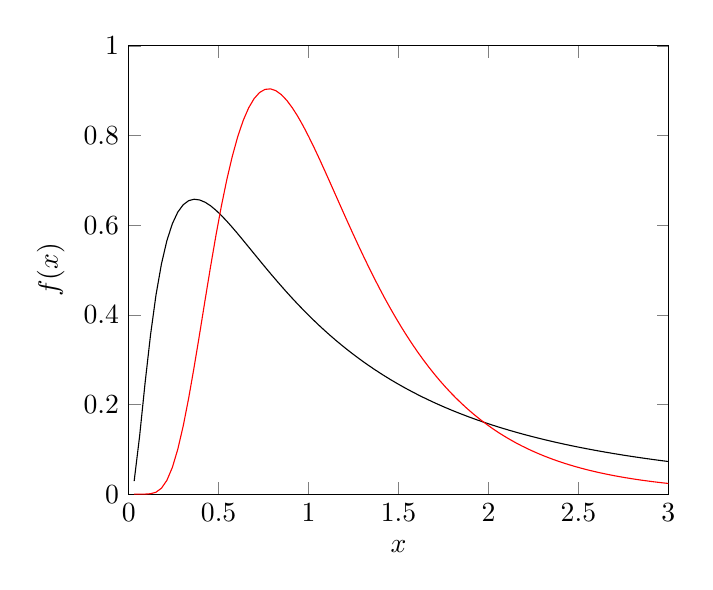
\begin{tikzpicture}
\begin{axis}[xlabel = $x$,
ylabel = {$f(x)$},
samples=100,
xmin=0, xmax=3,
ymin=0, ymax=1,
]

\addplot[color=black, domain=0:3]{1/(1*sqrt(2*pi)*x)*exp(-((ln(x))^2)/(2))};
\addplot[color=red, domain=0:3]{1/(1*sqrt(2*pi)*x*0.5)*exp(-((ln(x))^2)/(0.5))};

\end{axis}
\end{tikzpicture}
\caption{Density of $LN(0,1)$(black and $LN(0,0.5)$(red). Note the positive skewness.}
\end{figure}

\subsubsection{Extension to univariate lognormal distribution}

\begin{definition}\cite{borovkova2007closed}
\hfill
\begin{itemize}
	\item \textbf{regular log-normal distribution} with parameter $(\mu, \sigma^2)$ is given by
	$$f(x) = \frac{1}{x\sigma \sqrt{2\pi}}\exp(-\frac{(\ln x - \mu)^2}{2\sigma^2}),x>0.$$
	\item \textbf{negative log-normal distribution} with parameter $(\mu, \sigma)$, denoted by $NLN(\mu,\sigma^2)$ is given by
	$$f(x) = \frac{1}{x\sigma \sqrt{2\pi}}\exp(-\frac{(\ln -x - \mu)^2}{2\sigma^2}),x<0.$$
	\item \textbf{shifted log-normal distribution} with parameter $(\mu, \sigma,\tau)$,denoted by $SLN(\mu,\sigma^2,\tau)$ is given by
	$$f(x) = \frac{1}{(x-\tau)\sigma \sqrt{2\pi}}\exp(-\frac{(\ln x-\tau - \mu)^2}{2\sigma^2}),x>\tau.$$
	\item \textbf{negative shifted log-normal distribution} with parameter $(\mu, \sigma^2, \tau)$ is given by
	$$f(x) = \frac{1}{(-x-\tau)\sigma \sqrt{2\pi}}\exp(-\frac{(\ln (-x-\tau) - \mu)^2}{2\sigma^2}),x<-\tau.$$
\end{itemize}	
\end{definition}

\begin{figure}[H]
	\centering
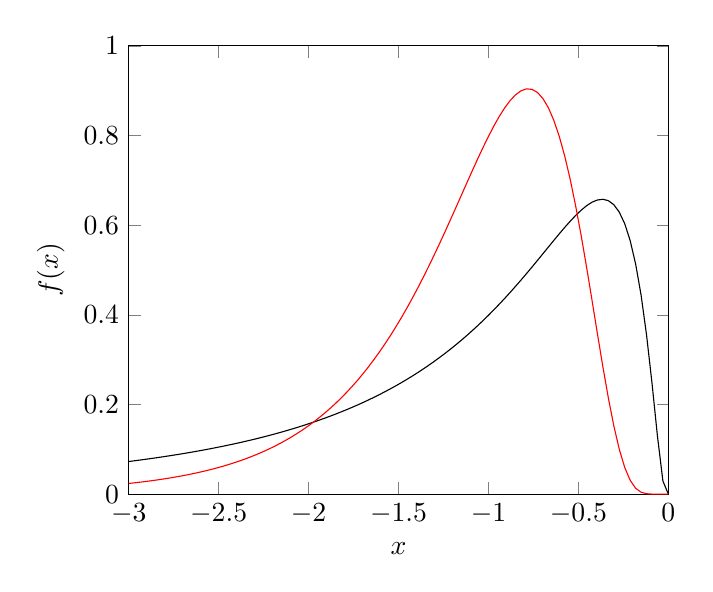
\begin{tikzpicture}
\begin{axis}[xlabel = $x$,
ylabel = {$f(x)$},
samples=100,
xmin=-3, xmax=0,
ymin=0, ymax=1,
]

\addplot[color=black, domain=-3:0]{-1/(1*sqrt(2*pi)*x)*exp(-((ln(-x))^2)/(2))};
\addplot[color=red, domain=-3:0]{-1/(1*sqrt(2*pi)*x*0.5)*exp(-((ln(-x))^2)/(0.5))};

\end{axis}
\end{tikzpicture}
	\caption{Density of $NLN(0,1)$(black and $NLN(0,0.5)$(red). Note the negative skewness.}
\end{figure}

\begin{lemma}
Let $X\sim LN(\mu,\sigma^2)$. It follows that
\begin{itemize}
	\item Let $Y = -X$. Then $Y\sim NLN(\mu, \sigma^2)$.
	\item Let $Z = X+\tau$. Then $Y\sim NLN(\mu, \sigma^2,\tau)$.
	\item Let $W = -X - \tau$. Then $Y\sim NSLN(\mu, \sigma^2, \tau)$.
\end{itemize}	
\end{lemma}
\begin{proof}
Straight forward from definition and transformation.
\end{proof}

\begin{lemma}[basic properties of shifted lognormal distribution]\label{ch:theory-of-statistics:th:BasicPropertyShiftedlognormalRandomVariable}
Let $X\sim SLN(\mu,\sigma^2,\tau)$. Then
\begin{itemize}
	\item $$E[X] = \tau + \exp(\mu+\frac{1}{2}\sigma^2).$$
	\item $$E[X^2] = \tau^2 + 2\tau\exp(\mu+\frac{1}{2}\sigma^2)+\exp(2\mu+2\sigma^2).$$
	\item $$E[X^3] = \tau^3 + 3\tau^2\exp(\mu+\frac{1}{2}\sigma^2)+3\tau\exp(2\mu+2\sigma^2)+\exp(3\mu+\frac{9}{2}\sigma^2).$$
\end{itemize}	
\end{lemma}
\begin{proof}
Note that from \autoref{ch:theory-of-statistics:th:meanVariancelognormalRandomVariable}, we have
if $Y\sim LN(\mu,\sigma^2)$, then $E[Y^m] = \exp(m\mu + \frac{1}{2}m^2\sigma^2)$.
Then, we use
$$E[X] = E[Y+\tau] = E[Y] + \tau,$$
$$E[X^2] = E[(Y+\tau)^2] = E[Y^2] + 2\tau E[Y] + \tau^2,$$
$$E[X^3] = E[(Y+\tau)^3] = E[Y^3] + 3\tau E[Y^2] + 3\tau^2 E[Y] + \tau^3.$$

\end{proof}

\subsubsection{Moment matching approximation}
\begin{lemma}[2 parameter Log-normal approximation via moment matching]\label{ch:theory-of-statistics:th:lognormalApproximationViaMomentMatching}
Suppose we have a random variable $X$ having moments given by
$$E[X] = M_1, E[X^2] = M_2.$$
Let $Y$ be a log-normal random variable defined by
$$Y = M_1\exp(-\frac{1}{2}v^2 + vZ), Z\in N(0,1),$$
where 
$$v^2 = \log(M_2/M_1^2)$$
Then $Y$ has the same first two moments as $X$; that is
$$E[Y] = M_1, E[Y^2] = M_2.$$
\end{lemma}
\begin{proof}
Using moment generating function of $Z$, we know that
$$E[Y] = M_Z(v)M_1\exp(-\frac{1}{2}v^2) = M_1.$$
and
$$E[Y^2] = M_Z(2v)M_1^2\exp(-v^2) = \exp(v^2)M_1^2=\frac{M_2}{M_1^2}M_1^2 = M_2.$$
\end{proof}


\begin{lemma}[3 parameter shifted lognormal approximation via moment matching]\label{ch:theory-of-statistics:th:ShiftedlognormalApproximationViaMomentMatching}
	Suppose we have a random variable $X$ having moments given by
	$$E[X] = M_1, E[X^2] = M_2, E[X^3] = M_3.$$
	Let $Y$ be a  shifted log-normal random variable with parameter $SLN(\mu,\sigma^2,\tau)$ such that
	$$E[Y] = \tau + \exp(\mu+\frac{1}{2}\sigma^2),$$
	$$E[Y^2] = \tau^2 + 2\tau\exp(\mu+\frac{1}{2}\sigma^2)+\exp(2\mu+2\sigma^2),$$
	$$E[Y^3] = \tau^3 + 3\tau^2\exp(\mu+\frac{1}{2}\sigma^2)+3\tau\exp(2\mu+2\sigma^2)+\exp(3\mu+\frac{9}{2}\sigma^2).$$
	
	
If we can find $(\mu,\sigma,\tau)$ such that
$$E[X] = E[Y], E[X^2] = E[Y^2],E[X^3] = E[Y^3],$$
then $X$ and $Y$ have matched moments.

\end{lemma}
\begin{proof}
For moments of $Y$, see \autoref{ch:theory-of-statistics:th:BasicPropertyShiftedlognormalRandomVariable}.
\end{proof}

\begin{note}[choice of approximating distribution]\cite{borovkova2007closed}
We can based on the target distribution's location and skewness to choose the type of lognormal distribution we want to use. The table is good summary.
	
	
\begin{center}
	\begin{tabular}{|c|c|c|c|c|}
		\hline
		skewness                & $\eta > 0$   & $\eta>0$   & $\eta<0$      & $\eta<0$         \\ \hline
		location                & $\tau\geq 0$ & $\tau < 0$ & $\tau \geq 0$ & $\tau < 0$       \\ \hline
		choice of approximation & regular      & shifted    & negative      & negative shifted \\ \hline
	\end{tabular}

\end{center}	
\end{note}

\subsubsection{Multivariate lognormal distribution}

\begin{definition}[multivariate lognormal distribution]\label{ch:theory-of-statistics:def:multivariateLognormalDistribution}
If $X=(X_1,X_2,...,X_n)\sim MN(\mu,\Sigma)$, then $Y=\exp(X)=(\exp(X_1),\exp(X_2),...,\exp(X_n)) \sim MLN(\mu, \Sigma)$,
i.e., $Y$ has multivariate lognormal distribution
\end{definition}

\begin{lemma}[basic properties of multivariate lognormal distribution]\label{ch:theory-of-statistics:th:BasicPropertiesMultivariateLognormal}
Let $X=(X_1,X_2,...,X_n)\sim MN(\mu, \Sigma)$ and $Y = \exp(X)=(\exp(X_1),\exp(X_2),...,\exp(X_n))$. Then
\begin{itemize}
	\item $E[Y_i] = \exp(\mu_i + \frac{1}{2}\Sigma_{ii})$.
	\item $E[Y_iY_j] = \exp(\mu_i+\mu_j + \frac{1}{2}(\Sigma_{ii} + \Sigma_{jj} + 2\Sigma_{ij})) = E[Y_i][Y_i]\exp(\Sigma_{ij}).$
	\item $Var[Y_i] = \exp(2\mu_i + \Sigma_{ii})(\exp(\Sigma_{ii}) - 1).$
	\item $Cov[Y_iY_j] = \exp(\mu_i+\mu_j + \frac{1}{2}(\Sigma_{ii} + \Sigma_{jj}))(\exp(\Sigma_{ij}) - 1).$
\end{itemize}	
	
\end{lemma}
\begin{proof}
(1)Note that $M_X(t) = \exp(t^T\mu + \frac{1}{2}t^T \Sigma t), t\in \R^n$, and $E[Y_i] = M_X(e_i)$.
(2) Let $t = e_i+e_j$. Then $$E[Y_iY_j] = M_X(t) = \exp(\mu_i+\mu_j + \frac{1}{2}(\Sigma_{ii} + \Sigma_{jj} + 2\Sigma_{ij})).$$
(3) $$Var[Y_i] = E[Y_iY_i]- E[Y_i]E[Y_i].$$
(4) $$Cov[Y_i,Y_j] = E[Y_iY_j]- E[Y_i]E[Y_j].$$
\end{proof}



\subsection{Exponential distribution}
\begin{definition}[exponential distribution]\index{exponential distribution}
	A random variable $X$ is said to have an exponential distribution $Exp(\lambda)$ with parameter $\lambda$ if it has pdf given as
	$$p(x|\lambda) = \lambda \exp(-\lambda x)$$
	with $x\in [0,\infty)$.	
\end{definition}

\begin{lemma}[basic properites]
	Let $X$ be a random variable with exponential distribution with parameter $\lambda$, then we have
	\begin{itemize}
		\item $E[X] = 1/\lambda$
		\item $Var[X] = 1/\lambda^2$
		\item memoryless: 
		$$P(X > s+t | X > s) = P(X>t)$$
		(even though $P(X>s+t) < P(X>t)$)
	\end{itemize}
\end{lemma}
\begin{proof}
(1)(2) are straightforward. (3) The cmf is given as
$$F(t) = \int_0^t \lambda\exp(-\lambda \tau) d\tau = 1-\exp(-\lambda t)$$
$$P(X>s+t|X>s) = \frac{P(X>s+t \cap X > s)}{P(X>s)} = \frac{P(X > s+t)}{P(X>s)} = \frac{\exp(-\lambda(s+t))}{\exp(-\lambda t)} = \exp(-\lambda t)$$
\end{proof}


\begin{remark}[interpretation of memorylessness]
Supppose we are waiting for an event to occur, and we model the waiting time as a random variable $X$ with $Exp(\lambda)$. If we already wait for $s$ time, the distribution that we need to wait an extra of $t$ time is the same as the distribution of the waiting time at time 0.
\end{remark}

\begin{remark}
\textbf{Exponential distribution is the only memoryless continuous distribution.}\cite{brzezniak1999basic}.
\end{remark}

\begin{lemma}[Normal approximate sum of Exponential]
	Let $X_1,...,X_n$ be independent iid random variable of $Exp(\lambda)$, then
	$$Y = \sum_{i=1}^n X_i$$
	can be approximated(when $n\to \infty$) by $$\frac{Y - n\mu}{\sqrt{n\sigma}}\sim N(0,1),$$
	where $\mu = n/\lambda$,and $\sigma = n/\lambda^2$.
\end{lemma}
\begin{proof}
	Directly from Central Limit Theorem(\autoref{ch:theory-of-probability:centralLimitTheorem}). Also see Gamma distribution properties, since exponential distribution is a special case of Gamma distribution.
\end{proof}


\subsection{Poisson distribution}
\begin{definition}[Poisson distribution]\index{Poisson distribution}
	A discrete random variable $X$ is said to have a Poisson distribution $Poisson(\lambda)$ with parameter $\lambda$ if it has pmf given as
	$$p(x) = \frac{\lambda^xe^{-\lambda}}{x!}$$
	with $x\in \{0,1,2,...\}$.	
\end{definition}


\begin{lemma}[basic property of Poisson distribution]\cite[154]{hoggintroduction}\label{ch:theory-of-statistics:th:PoissonBasicproperty}
Let $X$ be a random variable with distribution $Poisson(\lambda)$. Then
\begin{itemize}
	\item $M(t) = \exp(\lambda(e^t - 1))$.
	\item $E[X] = \lambda, Var[X] = \lambda.$
\end{itemize}
\end{lemma}
\begin{proof}
(1)
\begin{align*}
M_X(t) &= E[e^{tX}] \\
&= \sum_{n=0}^{\infty} e^{tn}\frac{\lambda^n}{n!}e^{-\lambda}\\
&= e^{-\lambda}\sum_{n=0}^{\infty} \frac{(\lambda e^t)^n}{n!}\\
&= e^{-\lambda}e^{\lambda e^t}.
\end{align*}
(2) $E[X] = M_X'(0) = \lambda, E[X^2] = M_X''(0) = \lambda^2-\lambda$.
\end{proof}


\begin{lemma}[sum of Poisson distribution]\label{ch:theory-of-statistics:th:sumofPoisson}
Assume $X_1,...,X_n$ to be independent random variables, and $X_i \sim Poisson(\theta_i),i=1,...,n$. Then $$Y = \sum_{i=1}^n X_i \sim Poisson(\sum_{i=1}^n \theta_i).$$
\end{lemma}
\begin{proof}
Note that $$M_Y(t) = \prod_{i=1}^n M_{X_i}(t) = \exp{\sum_{i=1}^n \theta_i(e^t - 1)}.$$
\end{proof}

\begin{lemma}[Normal approximate sum of Poisson]
Let $X_1,...,X_n$ be independent iid random variable of $Poisson(\theta)$, then
$$Y = \sum_{i=1}^n X_i$$
can be approximated by $$\frac{Y - n\theta}{\sqrt{n\theta}}\sim N(0,1),$$
or equivalently
$$Y \sim N(n\theta,n\theta).$$
\end{lemma}
\begin{proof}
Directly from Central Limit Theorem(\autoref{ch:theory-of-probability:centralLimitTheorem}).
\end{proof}

\subsection{Gamma distribution}
\begin{definition}[Gamma distribution]\cite[42]{murphy2012machine}\index{Gamma distribution}
A random variable $X$ is said to have a Gamma distribution $Gamma(a,b)$ with parameter $a,b$ if it has pdf given as
$$f(x) = \frac{b^a}{\Gamma(a)}x^{a-1}e^{-bx}$$
with support $x\in (0,\infty)$.	
\end{definition}

\begin{remark}[exponential distribution is a special case ]
An exponential distribution with parameter $b$ is a Gamma distribution $Gamma(1,b)$with 
$$f(x) = be^{-bx}.$$
\end{remark}

\begin{remark}[Application in arrival times of Poisson process]
If $N(t)$ is a Poisson process with rate $\lambda$, then the arrival time $T_1,T_2,...$ have $T_n\sim Gamma(n,\lambda)$ distribution.( See
	\autoref{ch:theory-of-stochastic-process:th:arrivaltimepoissonprocess})
\end{remark}

\begin{mdframed}
\textbf{Caution!}
Gamma distribution is different from Gamma function $\Gamma(t)$, which is given as
$$\Gamma(t) = \int_0^\infty x^{t-1}e^{-x}dx$$
\end{mdframed}

\begin{remark}[conjugate prior for Poisson distribution]
	Gammad distribution conjugate prior for the parameter of Poisson distribution. When integrate out $x$ in $\Gamma(t)$, we have
	$$ \int_0^\infty  x^{a-1}e^{-bx} dx = \Gamma(a)/b^2$$
\end{remark}

\begin{lemma}[mean and variance]
The Gamma distribution $Gamma(a,b)$ has mean $a/b$ and variance $a/b^2$.
\end{lemma}
\begin{proof}
Using the property of$$ \int_0^\infty  x^{a-1}e^{-bx} dx = \Gamma(a)/b^a,$$
we can show the result. 
\end{proof}


\begin{theorem}[sum of Gamma random variables]\cite[163]{hoggintroduction}\label{ch:theory-of-statistics:th:sumofGamma}
Let $X_1,...,X_n$ be independent random variables. Suppose $X_i \sim Gamma(a_i,b),\forall i=1,...,n$. Then
$$Y = \sum_{i=1}^n X_i \sim Gamma(\sum_{i=1}^n a_i,b)$$
\end{theorem}
\begin{proof}
This can be proved using moment generating functions.
\end{proof}

\begin{lemma}[Normal approximate sum of Gamma]
	Let $X_1,...,X_n$ be independent iid random variables of $Gamma(a,b)$, then
	$$Y = \sum_{i=1}^n X_i$$
	can be approximated(when $n\to \infty$) by $$\frac{Y - n\mu}{\sqrt{n\sigma}}\sim N(0,1),$$
	where $\mu = na/b$,and $\sigma = na/b^2$.
\end{lemma}
\begin{proof}
	Directly from Central Limit Theorem(\autoref{ch:theory-of-probability:centralLimitTheorem}).
\end{proof}

\subsection{Geometric distribution}
\begin{definition}[geometric distribution]\index{geometric distribution}
	A discrete random variable $X$ is said to have a geometric distribution $Geo(\theta)$ with parameter $\theta$ if it has pmf given as
	$$p(X=k) = (1-\theta)^{k-1}\theta$$
	with $k\in \{1,2,...\}$.	
\end{definition}

\begin{remark}[relation to Bernoulli trias]
The geometric distribution The probability distribution of the number X of Bernoulli trials needed to get one success, supported on the set { 1, 2, 3, ...}	
\end{remark}


\begin{lemma}[basic statistics of geometric distribution]\label{ch:theory-of-statistics:th:BasicStatistcsGeometricDistribution}
The expected value of a geometrically distributed random variable $X$ with parameter $p$ is $1/p$ and the variance is $(1-p)/p^2$.
\end{lemma}
\begin{proof}
(1)
	$$E[X] = \sum_{k=1}^\infty k(1-p)^{k-1}p $$
	$$(1-p)E[X] = \sum_{k=1}^\infty k(1-p)^{k}p $$
subtract and get $pE[X] = 1$.\\
(2) 	$$Var[X] = \sum_{k=1}^\infty (k-1/p)^2(1-p)^{k-1}p $$
can be proved similarly.
\end{proof}







\subsection{Binomial distribution}
\begin{definition}[binomial distribution]\index{binomial distribution}
	A discrete random variable $X$ is said to have a Binomial distribution $Binomial(n,p)$ with parameter $n,p$ if it has pmf given as
	$$f(X=k) = \binom{n}{k}p^k(1-p)^{n-k}$$
	with $x\in \{0,1,2,...,n\}$.
\end{definition}

\begin{remark}[interpretation]
Binomial distribution represents the probability distribution of the number of successes in a sequence of n independent binary experiments, each of which yields 1 with probability p.
\end{remark}  

\begin{remark}[relation to Bernoulli distribution]
Let $X_i$ be iid random variables with Bernoulli distribution of parameter $p$, then 
$$Y = \sum_{i=1}^n X_i$$ is a random variable of binomial distribution with parameter $(n,p)$. 
\end{remark}


\begin{lemma}[sum of independent binomial random variable]
Let $X_1,X_2,...,X_K$ be the independent binomial random variables with parameter $(n_1,p),(n_2,p),...,(n_K,p)$. Let
$Y = \sum_{i=1}^K X_i $. Then
\begin{itemize}
	\item $M_{X_i}(t) = (1-p + pe^t)^{n_i},i=1,...,K$.
	\item $M_Y(t) = (1-p + pe^t)^{\sum_{i=1}^K n_i}$
	\item $Y \sim Binomial(\sum_{i=1}^K n_i, p).$
\end{itemize}
\end{lemma}
\begin{proof}
(1) Use the mgf of Bernoulli distribution(\autoref{ch:theory-of-statistics:th:Bernoullidistributionproperty}).
(2)(3)
Consider $X_1\sim Binomial(n_1,p)$ and $X_2\sim Binomial(n_2,p)$, each has momemt generating function of $(1-p+pe^t)^{n_1}$ and $(1-p+pe^t)^{n_2}$. $X_1+X_2$ will have mgf of 
$(1-p+pe^t)^{n_1+n_2}$(\autoref{ch:theory-of-probability:th:additionandscalingtheoremformgf}), corresponding to $Binomial(n_1+n_2,p)$. It is straight forward to extend multiple cases. 
\end{proof}


\begin{lemma}[convergence of binomial distribution to Poisson distribution]
Suppose that $p_n\in (0,1)$ for $n\in \cN_+$ and $np_n\to \lambda$ as $n\to \infty$. Then the binomial distribution with parameters $n$ and $p_n$ converges to the Poisson distribution with parameter $\lambda$ \textbf{in distribution}  as $n\to \infty$. That is, for fixed $k\in \cN$, 
$$\binom{n}{k}p_n^k(1-p_n)^{n-k} \to e^{-\lambda}\frac{\lambda^k}{k!}$$
as $n\to \infty$.
\end{lemma}
\begin{proof}
(direct method)Note that
\begin{align*}
\binom{n}{k}p_n^k(1-p_n)^{n-k} &=\frac{n(n-1)(n-2)\cdots(n-k+1)}{k!}(p_n)^k(1-p_n)^{n-k} \\
&=\frac{n(n-1)(n-2)\cdots(n-k+1)}{k!}(\frac{\lambda}{n})^k(1-\frac{\lambda}{n})^{n-k} \\
&\approx\frac{n^k}{k!}(\frac{\lambda}{n})^k(1-\frac{\lambda}{n})^{n-k} \\
&=\frac{\lambda^k}{k!}(1-\frac{\lambda}{n})^{n-k}\\
&\to e^{-\lambda \frac{n-k}{n}} \frac{\lambda^k}{k!}\\
&\approx e^{-\lambda} \frac{\lambda^k}{k!}
\end{align*}

(use generating function)
Note that binomial distribution has probability generating function(\autoref{ch:theory-of-probability:def:probabilitygeneratingfunction})
$$((1-p_n)+p_ns)^n = (1 + (pns-p_n)n/n)^n \to e^{(s-1)a},n\to\infty$$
where $e^{(s-1)a}$ is the generating function of Poisson distribution.
\end{proof}

\begin{remark}[Poisson distribution as an approximate for large $n$ and small $k$]
Note that the lemma requires that $k$ fixed. In other words, when $n\gg k$, we can use Poisson distribution to approximate binomial distribution.
\end{remark}

\subsection{Hypergeometric distribution}
\begin{definition}[hypergeometric distribution distribution]\cite[148]{hoggintroduction}\index{hypergeometric distribution}
	A random variable $X$ is said to have a hypergeometric distribution $HG(N,K,n)$ with parameter $N,K,n$ if it has pmf given as
	$$p(x = k) = \frac{\binom{K}{k}\binom{N-K}{n-k}}{\binom{N}{n}} $$
	with support $x\in \{0,1,...,\min(n,K)\}$. Note that the parameters should be non-negative integers and satisfying $$N\geq K, N\geq n.$$

\end{definition}


\begin{remark}[interpretation]
	$p(x = k)$ describes the probability of  $k$ successes in  $n$ draws, without replacement, from a finite population of size $N$ that contains exactly $K$ successes.
\end{remark}

\begin{lemma}[combinatorial identities]
Assuming $K\geq n$, we have
	$$\sum_{0\leq k\leq n} \frac{\binom{K}{k}\binom{N-K}{n-k}}{\binom{N}{n}} = 1$$
\end{lemma}

\begin{lemma}[mean of a hypergeometric distribution]\cite[148]{hoggintroduction}
Let $X$ be a random variable with $HG(N,K,n)$, then its mean is
$$E[X] = n\frac{K}{N}$$
\end{lemma}



\subsection{Beta distribution}
\begin{definition}[Beta distribution]\cite[43]{murphy2012machine}\index{Beta distribution}
	A random variable $X$ is said to have a Beta distribution $B(a,b)$ with parameter $a,b$ if it has a pdf given as
	$$f(x) = \frac{x^{a-1}(1-x)^{b-1}}{B(a,b)},B(a,b)=\frac{\Gamma(a)\Gamma(b)}{\Gamma(a+b)}$$
	with support $x\in [0,1]$.
\end{definition}





\begin{remark}\hfill
	\begin{itemize}
		\item $$\int_0^1 x^{a-1}(1-x)^{b-1} dx = \frac{\Gamma(a)\Gamma(b)}{\Gamma(a+b)}$$
		\item Beta distribution is commonly \textbf{used as the conjugate prior for binomial distribution}, where
		$$p(y_1,...,y_n|\theta) = \theta^{\sum_i y_i}(1-\theta)^{n-\sum_i y_i},y_i\in \{0,1\}$$
		then the posterior distribution will also be Beta.
	\end{itemize}
\end{remark}



\begin{lemma}[basic property]\label{ch:theory-of-statistics:th:propertyBetaDistribution}
Let $X$ be a random variable with distribution $B(a,b)$.
	\begin{itemize}
		\item $$E[X] = \frac{a}{a+b}.$$
		\item $$E[X^2] = \frac{a(a+1)}{(a+b)(a+b+1)}.$$
		\item $$E[X^r] = \frac{a(a+1)\cdots (a+r-1)}{(a+b)(a+b+1)\cdots(a+b+r-1)}.$$
		\item $$Var[X] = \frac{ab}{(a+b)^2(a+b+1)}.$$
		\item The mode of $X$, i.e., the value $x$ that has the maximum probability is
		$$x^* = \frac{a-1}{a+b-2}.$$
	\end{itemize}
\end{lemma}
\begin{proof}
	(1)This can be proved using properties of Gamma distribution.
\begin{align*}
E[X] &= \int_0^1 xf(x)dx \\
&= \int_0^1 \frac{x^a(1-x)^{b-1}}{B(a,b)} \\
&= \frac{B(a+1,b)}{B(a,b)} \\
&= \frac{\Gamma(a+1)\Gamma(b)}{\Gamma(a+b+1)}/\frac{\Gamma(a)\Gamma(b)}{\Gamma(a+b)} \\
&= \frac{\Gamma(a+1)\Gamma(a+b)}{\Gamma(a+b+1)\Gamma(a)} \\
&= \frac{a}{a+b} 
\end{align*}	
	(2) \begin{align*}
	E[X^2] &= \int_0^1 x^2f(x)dx \\
	&= \int_0^1 \frac{x^{a+1}(1-x)^{b-1}}{B(a,b)} \\
	&= \frac{B(a+2,b)}{B(a,b)} \\
	&= \frac{\Gamma(a+2)\Gamma(b)}{\Gamma(a+b+2)}/\frac{\Gamma(a)\Gamma(b)}{\Gamma(a+b)} \\
	&= \frac{\Gamma(a+2)\Gamma(a+b)}{\Gamma(a+b+2)\Gamma(a)} \\
	&= \frac{a(a+1)}{(a+b)(a+b+1)} 
	\end{align*}
(3) Use $Var[X] = E[X^2] - E[X]^2.$
(4) To find the maximizer for $x^{a-1}(1-x)^{b-1}$, we take the log and maximize it. We have
$$\ln f(x) = (a - 1)\ln x + (b-1)\ln (1-x).$$
Take the derivative with respect to $x$ and set to 0, we have
\begin{align*}
\frac{a-1}{x} &= \frac{b-1}{1-x} \\
(a-1)(1-x) &= x(b-1) \\
\implies x^* = \frac{a-1}{a+b-2}.
\end{align*}
\end{proof}


\subsection{Multinomial distribution}
\begin{definition}\cite[35]{murphy2012machine}
A discrete random vector $X=(X_1,...,X_n)$ is said to have multinomial distribution with parameters $(p_1,...,p_n)$ and $m$ if its pmf is given as
$$f(x_1,x_2,...,x_n)=\frac{m!}{x_1!...x_n!}p_1^{x_1}...p_n^{x_n}$$
where we require $x_i\in \{0,...,m\}$,$\sum x_i = m,\sum p_i=1$.
\end{definition}

\begin{remark}
	Consider $m$ independent experiment, each has $n$ outcomes with probability $p_i$ to occur. The outcome distribution is given as\cite{casella2002statistical}
	$$
	f(x_1,x_2,...,x_n)=\frac{m!}{x_1!...x_n!}p_1^{x_1}...p_n^{x_n}
	$$
	where $\sum x_i = m,\sum p_i=1$.
\end{remark}



\begin{lemma}[basic properties of Multinomial Distribution]\label{ch:theory-of-statistics:th:propertyMultinomialDistribution}
Let $X=(X_1,...,X_n)$ discrete random vector with multinomial distribution with parameters $p=(p_1,...,p_n)$ and $m$.
	\begin{itemize}
		\item 
		\item $$E[X_i] = np_i.$$
		\item $$Var[X_i] = np_i(1-p_i), Cov(X_i,X_j) = np_i(1-p_i),$$
	or in vector form
	$$Var[X] = n(diag(p) = pp^T).$$	
	\end{itemize}
\end{lemma}
\begin{proof}
	(1)This can be proved using properties of Gamma distribution.
	\begin{align*}
	E[X_i] &= \int_0^1 x_if(x)dx \\
	&=  \frac{\prod_{k=1}^K \Gamma(a_k + \delta_{ik})}{\Gamma(a_0+1)}/\frac{\prod_{k=1}^K \Gamma(a_k)}{\Gamma(a_0)}\\
	&= \frac{a_i}{a_0}
	\end{align*}	
	(2) \begin{align*}
	E[X_i^2] &= \int_0^1 x^2_if(x)dx \\
	&=  \frac{\prod_{k=1}^K \Gamma(a_k + 2\delta_{ik})}{\Gamma(a_0+2)}/\frac{\prod_{k=1}^K \Gamma(a_k)}{\Gamma(a_0)}\\
	&= \frac{a_i(a_i+1)}{(a_0+1)a_0}  
	\end{align*}
	(3) Use $Var[X] = E[X^2] - E[X]^2.$
	(4) To find the maximizer for $f(x)$, we take the log and maximize it. The optimality condition requires that $x_i^*\propto a_i-1$ and $\sum_{i=1}^{K}a_i=1$.
\end{proof}

\subsection{Dirichlet distribution}
\begin{definition}\cite[49]{murphy2012machine}
	A random vector $X=(X_1,...,X_K)$ is said to have a Dirichlet distribution distribution with parameter $a=(a_1,...,a_K)$ if it has pdf given as
	$$f(x_1,...,x_K) = \frac{1}{B(a)} \prod_{k=1}^K x_k^{a_k-1}$$
	with support $x\in \{x:0\leq x_k\leq 1,\sum_k x_k = 1,\forall k=1,2...,K\}$, and $B(a)$ is a normalization constant given as
	$$B(a) = \frac{\prod_{k=1}^K \Gamma(a_k)}{\Gamma(\sum_k a_k)},$$
where $\Gamma(\cdot)$ is the Gamma function. 	
\end{definition}


\begin{remark}\hfill
\begin{itemize}
	\item Dirichlet distribution can be viewed as multivariate generalization of Beta distribution.
	\item Dirichlet distribution is usually \textbf{used as the conjugate prior} for multinomial distribution.
\end{itemize}	
\end{remark}


\begin{lemma}[basic properties of Dirichlet Distribution]\label{ch:theory-of-statistics:th:propertyDirichletDistribution}
	Let $X = (X_1,X_2,...,X_K),x_i\in (0,1), \sum_{i=1}^{K} x_i = 1$, be a random vector  with distribution $B(a),a\in \R^K$. Let $a_0 = \sum_{i=1}^{K}a_i$.
	\begin{itemize}
		\item $$E[X_i] = \frac{a_i}{\sum_{i=1}^{K} a_i}.$$
		\item $$E[X^2_i] = \frac{a_i(a_i+1)}{(a_0)(a_0+1)}.$$
		\item 
		$$Var[X_i] = \frac{a_i(a_0-a_i)}{a_0^2(a_0+1)}.$$
		\item The mode of $X$, i.e., the value $x$ that has the maximum probability is
		$$x^*_i = \frac{a_i-1}{a_0-K}.$$
	\end{itemize}
\end{lemma}
\begin{proof}
	(1)This can be proved using properties of Gamma distribution.
	\begin{align*}
	E[X_i] &= \int_0^1 x_if(x)dx \\
	&=  \frac{\prod_{k=1}^K \Gamma(a_k + \delta_{ik})}{\Gamma(a_0+1)}/\frac{\prod_{k=1}^K \Gamma(a_k)}{\Gamma(a_0)}\\
	&= \frac{a_i}{a_0}
	\end{align*}	
	(2) \begin{align*}
	E[X_i^2] &= \int_0^1 x^2_if(x)dx \\
&=  \frac{\prod_{k=1}^K \Gamma(a_k + 2\delta_{ik})}{\Gamma(a_0+2)}/\frac{\prod_{k=1}^K \Gamma(a_k)}{\Gamma(a_0)}\\
&= \frac{a_i(a_i+1)}{(a_0+1)a_0}  
	\end{align*}
	(3) Use $Var[X] = E[X^2] - E[X]^2.$
	(4) To find the maximizer for $f(x)$, we take the log and maximize it. The optimality condition requires that $x_i^*\propto a_i-1$ and $\sum_{i=1}^{K}a_i=1$.
\end{proof}

\subsection{$\chi^2$-distribution}
\subsubsection{Basic properties}
\begin{definition}
A random variable $X$ is said to have a $\chi^2(n)$ distribution with parameter $n\in \Z_+$ if it has pdf given as
$$f(x) = \frac{1}{2^{n/2}\Gamma(n/2)}x^{n/2-1}e^{-y/2}$$
with $x\in (0,+\infty)$	
\end{definition}

\begin{remark}[special case of Gamma distribution]
	$\chi^2(n)$ has the same distribution of Gamma(n/2,2).
\end{remark}

\begin{definition}[alternative]\index{$\chi^2$-distribution}
The $\chi^2$-distribution with $k$ degrees of freedom is the distribution of a sum of squares of $k$ independent standard normal random variables. Mathematically, if $X_1,X_2,..., X_k$ are iid random variable with $X_i\sim N(0,1)$, the random variable $$Q=\sum_{i=1}^k X_i^2$$ is distributed according to the $\chi^2$ distribution with $k$ degrees of freedom, writen as $Q\sim \chi^2(k)$.	
\end{definition}

\begin{lemma}[basic property]\cite[161-163]{hoggintroduction}\label{ch:theory-of-statistics:th:propertychisquare}
	Let $X_1,X_2$ be independent random variables. Suppose $X_1 \sim \chi^2(a_1),X_2\sim \chi^2(a_2)$. Then
	\begin{itemize}
		\item $Y = X_1+X_2 \sim \chi^2(a_1+a_2)$
		\item $\lambda X_1 \sim \lambda^2 \chi^2(a_1)$
		\item The moment generating function is given by
		$$M(t) = (1 - 2t)^{-r/2}.$$
	\end{itemize}
\end{lemma}
\begin{proof}
(1)This can be proved using properties of Gamma distribution.
(2) $\lambda X_1$ can be viewed as the sum of squares of normal random variables $Y_i$ with $N(0,\lambda^2)$.
Then $\sum_{i=1}^n (Y_i/\lambda)^2 \sim \chi^2(n) $. 
 
\end{proof}



\begin{lemma}[expectation and variance]\label{ch:theory-of-statistics:th:chi_expectationvariance}
Let random variable $X$ has distribution of $\chi^2(n)$, then
$$E[X] = n, Var[X] = 2n$$ 
In particular, $$E[X/n] = 1, Var[X/n] = 0 ~as~ n\to \infty.$$
that is the random variable $X/n$ becomes deterministic constant as $n\to \infty$.
\end{lemma}
\begin{proof}
(1)Let $Z\sim \chi^2(1), Z = Y^2, Y\sim N(0,1)$, then $E[Z] = Var[Y] + (E[Y])^2 = 1$.
$Var[Z] = E[Z^2] - (E[Z])^2 = E[Y^4] - 1 = 3 - 1 =2.$
(2) Use linearity of expectation that $E[X/n] = E[X]/n = 1$. Use $Var[X/n] = Var[X]/n^2 = 2/n$.
\end{proof}



\subsubsection{Quadratic forms and chi-square distribution}
\begin{definition}[quadratic forms of random vectors]\cite[485]{hoggintroduction}
Let $X=(X_1,X_2,...,X_n)^T$ be a random vector, we called $$Q = X^T\Sigma X,\Sigma\in \R^{n\times n},$$
a quadratic form of random vector  $X$.

Note that $Q$ is also a random variable.
\end{definition}

\begin{lemma}
Let $X$ be a $m$-dimensional random vector with multivariate Gaussian distribution, i.e., $X\sim N(\mu, \Sigma)$. It follows that
\begin{itemize}
	\item $$\Sigma^{1/2}(x-\mu)\sim N(0, I).$$
	\item $$(x-\mu)\Sigma^{-1}(x-\mu)\sim \chi^2(m).$$
\end{itemize}	
\end{lemma}
\begin{proof}
(1) Directly from affine transformation property of multivariate Gaussian random variable (\autoref{ch:theory-of-statistics:th:affinetransformmultivariatenormal}). 
(2) Use the definition that sum of iid normal random variable square is chi-square random variable.
\end{proof}


\begin{theorem}[chi-square orthogonal decomposition]\label{ch:theory-of-statistics:th:chi-squareOrthogonalDecomposition}
Let $X_1,X_2,...,X_n$ be independent standard normal variables such that 
$$\sum_{i=1}^n X_i^2 \sim \chi^2(n). $$
Denote $X = (X_1,...,X_n)^T$.
If there exists an orthogonal projector	$P\in \R^{n\times n}$ such that $Y = PX, Z = (I-P)X$, then
\begin{itemize}
	\item $Y \sim MN(0,P), Z\sim MN(0, I-P)$, and $Y,Z$ are independent of each other.  
	\item $Y^TY \sim \chi^2(r), r = rank(P)$; or equivalently, the quadratic form $Q = X^TPX\sim \chi^2(r)$.
	\item $Z^TZ \sim \chi^2(n-r)$;or equivalently, the quadratic form $Q = X^T(I-P)X\sim \chi^2(n-r)$
\end{itemize} 
In summary, for a quadratic form $Q = X^T\Sigma X$, if $\Sigma$ is idempotent and symmetric, then $Q\sim \chi^2(rank(\Sigma))$.
\end{theorem}
\begin{proof}
(1) From affine transform of multivariate normal(\autoref{ch:theory-of-statistics:th:affinetransformmultivariatenormal}), $$Y\sim MN(0, P\Sigma_X P^T) = MN(0, P^2) = MN(0,P).$$
To show independence, we have $E[YZ^T] = E[PXX^T(I-P)^T] = E[P(I-P)] = 0$.

(2) Let $U$ be the eigen-decomposition of $P$ such that $P = UU^T$. Let $Z = U^TX, Z\in \R^r, Z\sim MN(0, I_r)$. Let $V$  be the eigen-decomposition of $I-P$ such that $I-P = VV^T$. Let $W = V^TX, W\in \R^{n-r}, W\sim MN(0, I_{n-r})$. We want to show that the characteristic function of the random quantity $Y^TY$ is the same as the characteristic function of $\chi^2(r)$. 
\begin{align*}
&E[\exp(itY^TY)] \\
=&\frac{1}{(2\pi)^{n/2}}\int\int\cdots \int \exp(it(U^TX)^T(U^TX) \exp(-\frac{1}{2}X^T(I-P + P) X))dx_1dx_2\cdots dx_n \\
=&\frac{1}{(2\pi)^{n/2}}\int\int\cdots \int \exp(itZ^TZ) \exp(-\frac{1}{2}(Z^TZ + W^TW))dz_1\cdots dz_r dw_{r+1}\cdots dw_n \\
=&\frac{1}{(2\pi)^{r/2}}\int\int\cdots \int \exp(itZ^TZ) \exp(-\frac{1}{2}(Z^TZ))dz_1\cdots dz_r
\end{align*}
where we change the integral variable such that $$[dz_1\cdots dz_r dw_{r+1}\cdots dw_n]^T = [U~ V](dx_1 dx_2 \cdots dx_n)^T$$. The last line is the characteristic function of  $\chi^2(r)$.
(3) similar to (2).
\end{proof}


\begin{lemma}[moment generating functions for Gaussian quadratic forms]\cite[523]{hoggintroduction}\label{ch:theory-of-statistics:th:momentGeneratingFunctionGaussianQuadraticForm}
Let $X=(X_1,X_2,...,X_n)^T$ where $X_1,X_2,...,X_n$ are iid $N(0,1)$. Consider the quadratic form $Q = X^TAX$ for a symmetric matrix $A$ of rank $r\leq n$. 
It follows that
\begin{itemize}
	\item $Q$ has the moment generating function $M(t) = \prod_{i=1}^r (1 - 2t\lambda_i)^{-1/2} = \abs{I - 2tA}^{-1/2},$
	where $\lambda_1,\lambda_2,...,\lambda_r$ are the nonzero eigenvalues of $A$, $\abs{t} < \frac{1}{\max \abs{\lambda_i}}.$
	\item If $A$ is an orthogonal projector such that $\lambda_1=\lambda_2=\cdots = \lambda_r = 1$, then
	$$M(t) = M_{\chi^2(r)}.$$
\end{itemize}
\end{lemma}
\begin{proof}
(1)Let the eigen-decomposition of $A$ be $$A = U\Lambda U^T, U\in \R^{n\times r}, \Lambda \in \R^{r\times r}.$$
Then 
$$Q = X^TAX = X^TU\Lambda U^TX = X^T(\sum_{i=1}^r \lambda_i u_iu_i^T) X =\sum_{i=1}^r \lambda_i (u_i^T X)^T.$$
Let $Y_i=u_i^T X,i=1,2,...,r$. It can be shown that $Y_i\sim N(0,1), E[Y_iY_j] = u_i^T E[XX^T]u_j^T = \delta_{ij}$; that is $Y_1,Y_2,...,Y_r \sim MN(0,I_r).$ 
Therefore, $Y_i^2 \sim \chi^2(1).$

The moment generating function is given by
\begin{align*}
M(t) &= E[\exp(tQ )] \\
&= E[\exp(t \sum_{i=1}^r \lambda_i Y_i^2 )] \\
&= \prod_{i=1}^r E[\exp(t \lambda_i Y_i^2 )] \\
&= \prod_{i=1}^r M_{\chi^2(1)}(\lambda_it) \\
& = \prod_{i=1}^r (1 - 2\lambda_i t)^{-1/2}
\end{align*}
where we use the moment generating function of $\chi^2(1)$ from \autoref{ch:theory-of-statistics:th:propertychisquare}.
(2) straight forward. 
\end{proof}



\begin{lemma}[independence of quadratic forms]\label{ch:theory-of-statistics:th:independenceOfChiSquareQuadraticForms}\cite[528]{hoggintroduction}
Let $X=(X_1,X_2,...,X_n)$ be a random vector where $X_1,X_2,...,X_n$ are iid $N(0,1)$. For real symmetric matrices $A,B\in \R^{n\times n}$, let $Q_1 = X^TAX$ and $Q_2 = X^TBX$. Then $Q_1$ and $Q_2$ are independent if and only if $AB = 0$.	
\end{lemma}
\begin{proof}
Let $rank(A) = r, rank(B) = s$. Let the eigendecomposition of $A,B$ be such that
$$A = \sum_{i=1}^r \lambda_i u_iu_i^T,A = \sum_{i=1}^s 
\beta_i v_iv_i^T.$$
If $AB = 0$, then $u_1,...,u_r, v_1,...,v_r$ will be orthogonal to each other. Then
$$Q_1+Q_2 = \sum_{i=1}^{r+s} \lambda_i u_iu_i^T,$$
where $u_{r+i} = v_i, \lambda_{r+i} = \beta_i$.

It is easy to see that(\autoref{ch:theory-of-statistics:th:momentGeneratingFunctionGaussianQuadraticForm}) 
$$M_{Q_1,Q_2}(t_1,t_2) = M_{Q_1}(t_1)M_{Q_2}(t_2).$$
Then from independence-from-mgf(\autoref{ch:theory-of-probability:th:IndependenceFromMomentGeneratingFunction}), we can prove $Q_1$ and $Q_2$ are independent.
	
\end{proof}

\subsubsection{Noncentral chi-squared distribution}
\begin{definition}[noncentral chi-squared distribution] Let $(X_1,X_2,...,X_k)$ be $k$ independent, normally distributed random variables with mean $\mu_i$ and unit variances. Then the random variable 
	$$Y = \sum_{i=1}^{k}X_i^2$$
is distributed according to the \textbf{noncentral chi-squared distribution} with parameter $k$ specifying the degree of freedom and $\lambda$, known as the \textbf{noncentrality parameter}, given by
$$\lambda = \sum_{i=1}^k \mu_i^2.$$	
\end{definition}

\subsection{Wishart distribution}\index{Wishrt distribution}
\begin{definition}[Wishart distribution]
	Let $X_1,...,X_n$ be independent $p$ dimensional multivariate normal random vector with distribution $MN(0,V)$. Let $X = [X_1,...,X_n]$. Then $M = XX^T$ is said to have Wishart distribution with parameter $(n,p,V)$.
\end{definition}

\begin{definition}[Wishart distribution]
	A random matrix $M\in \R^{p\times p}$ is said to have the Wishart distribution with parameters $W_p(n,V)$ if it has pdf 
	$$f(M) = \frac{1}{2^{np/2}\Gamma_p(\frac{n}{2}\abs{V}^{n/2})}\abs{M}^{n-p-1/2}\exp(\frac{1}{2}Tr[V^{-1}M]),$$
	with the support $M$ be the set of all symmetric positive definite matrices. Here $\Gamma_p(\alpha)$ is the multivariate gamma function. 	
\end{definition}


\begin{lemma}[basic properties]\hfill
	\begin{itemize}
		\item (reduction to $\chi^2$) If $M\in \R^{1\times 1}$, then
		$$M\sim W_1(n, \sigma^2) = \sigma^2 \chi^2(n).$$
		\item For $M\sim W_p(n,V)$, then $B^TMB \sim W_m(n,B^TVB)$, where $B\in \R^{p\times m}$.
		\item For $M\sim W_p(n,V)$, then $V^{-1/2}MV^{-1/2} \sim W_m(n,I).$
		\item If $M_i$ are independent $W_p(n_i,V)$, then $\sum_{i=1}^k \sim W_p(\sum_{i=1}^k n_i,V)$.
		\item If $M\sim W_p(n,V)$, then $E[M] = nV$.
		\item If $M_1,M_2$ are independent and $M_1+M_2 = M\sim W_p(n,V)$. Further if $M_1\sim W_p(n_1,V)$, then $M_2\sim W_p(n-n_1,V)$.
	\end{itemize}
\end{lemma}


\begin{lemma}[sample covariance]\index{sample covariance}
	The sample covariance
	$$\hat{Cov} = \frac{1}{n-1}\sum_{i=1}^n (X_i - \mean{X})(X_i-\mean{X})^T$$
	where $X_i$ are iid $MN(0,V)$, and $\mean{X} = \frac{1}{n}\sum_{i=1}^n X_i$, has the property of
	$$E[\hat{Cov}] = V.$$
\end{lemma}



\subsection{ $t$-distribution}\label{ch:theory-of-statistics:sec:studentTdistribution}
\subsubsection{Standard $t$ distribution}
\begin{definition}[t distribution]\cite[192]{hoggintroduction}
	A random variable $X$ is said to have a $t(n)$ distribution with parameter $n\in \Z_+$ if it has pdf given as
	$$f(x) = \frac{\Gamma((n+1)/2)}{\Gamma(n/2)\sqrt{\pi n}} (1 + \frac{t^2}{n})^{-(n+1)/2}$$
	with $x\in (-\infty,+\infty)$	
\end{definition}




\begin{definition}[alternative]\index{ $t$-distribution}\label{ch:theory-of-statistics:def:tdistribution}
Let random variable $W \sim N(0,1)$, Let random variable $V\sim \chi^2(n)$ \textbf{independent of} $V$. Define a new random variable $T$ as 
$$T=\frac{W}{\sqrt{V/n}}$$
Then $T$ has a $t$-distribution with degree of freedom $n$, denoted by $T_n$ or $t_n$.	
\end{definition}


\begin{remark}[comparison with normal distribution]\hfill
	\begin{itemize}
		\item $t$ distribution generally have shorter peak and fatter tails than normal distribution.
		\item $t_n \to N(0,1)$ as $n\to \infty$.
	\end{itemize}
\end{remark}

\begin{lemma}[mean and variance of $t$-distribution]
The mean for a $t$-distribution with degree of $n$ is given by
$$E[t_n] = \begin{cases}
0, n > 1 \\
\infty (undefined), n=1
\end{cases}.$$ 

The variance for a $t$-distribution with degree of $n$ is given by
$$Var[t_n] = \begin{cases}
\frac{n}{n-2}, n > 2 \\
\infty, n=1,2
\end{cases}.$$ 
\end{lemma}

\subsubsection{classical t distribution}
\begin{definition}\cite[95]{ruppert2015statistics}
If $Y$ has a standard $t_n$ distribution, then $$Z = \mu + \lambda Y$$
is said to have a $t_n(\mu,\lambda^2)$ distribution.
\end{definition}

\begin{lemma}[mean and variance of classical $t$-distribution]
Let $Z$ be a random variable $t_n(\mu,\lambda^2)$. Then
	$$E[Z] = \begin{cases}
	\mu, n > 1 \\
	\infty (undefined), n=1
	\end{cases},$$ 
and	
	
	$$Var[Z] = \begin{cases}
	\lambda^2\frac{n}{n-2}, n > 2 \\
	\infty, n=1,2
	\end{cases}.$$ 
\end{lemma}

\subsubsection{Multivariate $t$ distribution}
\begin{definition}[multivariate $t$ distribution]\cite{ruppert2015statistics}\label{ch:theory-of-statistics:def:MultivariateTDistribution}\hfill
\begin{itemize}
	\item Let $Z$ be a $d$ dimensional multivariate Gaussian $MN(0,\Sigma)$, and $\mu \in \R^d$. The $d$ dimensional random vector $Y$, defined as, $$X = \mu + \sqrt{\frac{n}{W}}Z,$$
	where $W\sim \chi^2(n)$ and $W$ is \textbf{independent} of $Z$,
	has a $t_n(\mu,\Sigma)$ multivariate distribution.
	\item Let $X \sim t_n(\mu, \Sigma)$. Then $X$ has the density given by
	$$f(x) = \frac{\Gamma((n+d)/2)}{\Gamma(n/2)n^{d/2}\pi^{d/2}\abs{\Sigma}^{1/2}}(1 + \frac{1}{n}(x-\mu)^T\Sigma^{-1}(x-\mu))^{-(n+d)/2}.$$
\end{itemize}	

\end{definition}

\begin{lemma}[mean and variance of multivariate $t$-distribution]
	Let $Z$ be a random variable $t_n(\mu,\Sigma)$. Then
	$$E[Z] = \begin{cases}
	\mu, n > 1 \\
	\infty (undefined), n=1
	\end{cases},$$ 
	and	
	
	$$Cov[Z] = \begin{cases}
	\Sigma\frac{n}{n-2}, n > 2 \\
	\infty, n=1,2
	\end{cases}.$$ 
\end{lemma}


\subsubsection{Student's Theorem}

\begin{theorem}[Student's Theorem]\cite[194]{hoggintroduction}\label{ch:theory-of-statistics:th:studentTheorem}\index{Student's theorem}
	Let $X_1,X_2,...,X_n$ be iid random variables each having a normal distribution with mean $\mu$ and variance $\sigma^2$. Define random variables as:\cite{hoggintroduction}
	$$\bar{X} = \frac{1}{n}\sum_{i=0}^nX_i, S^2=\frac{1}{n-1}\sum_{i=1}^n(X_i-\bar{X})^2 $$
	\begin{enumerate}
		\item $\bar{X}$ has a $N(\mu,\sigma^2/n)$ distribution
		\item $\bar{X}$ and $S^2$ are independent.
		\item $(n-1)S^2/\sigma^2$ has a $\chi^2(n-1)$ distribution
		\item The random variable $$T = \frac{\bar{X}-\mu}{S/\sqrt{n}}$$ has $t$-distribution with $n-1$ degrees of freedom.
	\end{enumerate}	
\end{theorem}
\begin{proof}
	(1)From \autoref{ch:theory-of-statistics:th:basicnormalproperties}. (2)
	We can prove $\mean{X}$ and the random vector $Y=(X_1-\mean{X},...,X_n-\mean{X})$ are independent. Note that
	$$\mean{X} = \frac{1}{n}\bm{1}^TX, Y = (I - \frac{1}{n}\bm{1}\bm{1}^T)X,$$
	and hence $\mean{X}$ and $Y$ are both normal. 
	\begin{align*}
	Cov(\mean{X},Y) &= X^T(\frac{1}{n}\bm{1}^T(I -\frac{1}{n}\bm{1}\bm{1}^T))X \\
	&=X^T\frac{1}{n}(\bm{1}^T - \frac{1}{n}\bm{1}^T\bm{1}\bm{1}^T)X \\
	&=X^T\frac{1}{n}(\bm{1}^T - \bm{1}^T))X = 0
	\end{align*}
	where we use the fact that $\bm{1}^T\bm{1} = n$.
	
	
	
	Then $S^2 = \frac{1}{n-1}Y^TY$ will be independent of $\mean{X}$ because $S^2$ is a function of $Y$(\autoref{ch:theory-of-probability:th:functionCompositionPreservesRandomVariableIndependence}).
	(3) See reference and \autoref{ch:theory-of-statistics:th:samplevariancedistribution}. (4) From the definition of the t distribution, we have
	$$Y=\frac{\bar{X}-\mu}{\sigma/\sqrt{n}}$$
	is the $N(0,1)$. $W=(n-1)S^2/\sigma^2$ has a $\chi^2(n-1)$ distribution. 
	Then 
	$$\frac{Y}{\sqrt{W/n-1}}$$ has $t(n-1)$ distribution.
\end{proof}

\subsection{ $F$-distribution}
\begin{definition}[$F$ distribution]\cite[192]{hoggintroduction}
	A random variable $X$ is said to have a $F(n_1,n_2)$ distribution with parameter $n_1,n_2\in \Z_+$ if it has pdf given as
	$$f(x) = \frac{\Gamma((n_1+n)2)/2)(n_1/n_2)^{n_1/2}y^{n_1/2 - 1}}{\Gamma(n_1/2)\Gamma(n_2/2)[1+(n_1x/n_2)]^{(n_1+n_2)/2}}$$
	with $x\in (0,+\infty)$	
\end{definition}


\begin{definition}[alternative]\index{$F$-distribution}
Given two \textbf{independent} chi-squared random variables $W$ and $V$ having $r_1$ and $r_2$ degrees of freedom. We define a new random variable $$W=\frac{U/r_1}{V/r_2}$$
Then $W$ has a $F$-distribution with parameter $(r_1,r_2)$.	
\end{definition}

\begin{lemma}[inverse relationship]
Let $X$ be a random variable with distribution $F(n_1,n_2)$, then $1/X$ is a random variable with distribution $F(n_2,n_1)$.	
\end{lemma}
\begin{proof}
	Directly from definition.
\end{proof}


\begin{lemma}[relationship to $t$ distribution]
	Let $X$ be a random variable with standard $t$ distribution with $n$ degrees of freedom. Then
	$$X^2 \sim F(1,n).$$
	That is, $X^2$ has the distribution of $F(1,n)$.
\end{lemma}
\begin{proof}
	Directly from definition.
\end{proof}



\begin{definition}[noncentral F distribution]\index{noncentral F distribution} Given two chi-squared random variables $W$ and $V$ such that $V$ is a noncentral chi-squared random variable with non-centrality parameter $\lambda$ and degree of freedom $r_1$, and $W$ is a chi-squared random variable having $r_1$ $r_2$ degrees of freedom. We define a new random variable $$W=\frac{U/r_1}{V/r_2}$$
	Then $W$ has a noncentral $F$-distribution  with parameter $(\lambda, r_1,r_2)$.	.
\end{definition}

\subsection{Empirical distributions}


\begin{definition}[empirical cumulative distribution function(CDF)]
	Given $N$ iid random variables $Y_1,Y_2,...,Y_N$ with common cdf $F(t)$, the empirical CDF is defined by
	$$\hat{F}_N(t) = \frac{number~of~elements~in~the~sample \leq t}{N} = \frac{1}{N}\sum_{i=1}^N \bm{1}_{Y_i \leq t}$$.	
\end{definition}

\begin{lemma}[basic statistic properties]
Let $\hat{F}_N(t)$ be the empirical cdf of a random sample of size $N$. For a fixed $t$, we have
\begin{itemize}
	\item $N\hat{F}_N(t)$ is a binomial random variable with parameter $(N,p)$,where $p = F(t)$.
	\item $N\hat{F}_N(t)$ is an unbiased estimator for $NF(t)$.
	\item $N\hat{F}_N(t)$ has variance $NF(t)(1 - F(t))$.
\end{itemize}	
\end{lemma}
\begin{proof}
(1) Note that based on the definition of $\hat{F}_N(t)	\frac{1}{N}\sum_{i=1}^N \bm{1}_{Y_i \leq t}$, $\bm{1}_{Y_i \leq t}$ is a Bernoulli random variable with parameter $p = F(t)$. Therefore,  $N\hat{F}_N(t) = \sum_{i=1}^N \bm{1}_{Y_i \leq t}$ will follow a binomial distribution of parameter $(N,p)$.
(2) $$E[N\hat{F}_N(t) ] = Np = NF(t).$$ 
(3) $$Var[N\hat{F}_N(t) ] = Np(1 - p) = NF(t)(1-F(t)).$$
\end{proof}

\subsection{Heavy-tailed distributions}
\subsubsection{Basic characterization}
\begin{definition}[Heavy-tailed distribution]\index{Heavy-tailed distribution}
The distribution of a random variable $X$ with distribution function $F$ is said to have a heavy right tail if
$$\lim_{x\to \infty} e^{\lambda x} Pr(X>x) = \infty, \forall \lambda > 0.$$
\end{definition}

\begin{remark}[interpretation]
Heavy-tailed distributions have densities decaying  slower in the tails than the normal. 
\end{remark}

\subsubsection{Pareto and power distribution}

\begin{definition}[Pareto distribution]
A random variable $X$ is said to have Pareto distribution with scale parameter $x_m > 0$ and shape parameter $\alpha > 0$ if its has pdf
$$f_X(x) = \begin{cases*}
\frac{\alpha x_m^\alpha}{ x^{\alpha + 1}}, x\geq x_m,\\
0, x < x_m.
\end{cases*};$$
or cdf
$$f_X(x) = \begin{cases*}
1 - (\frac{\alpha x_m}{ x})^\alpha, x\geq x_m,\\
0, x < x_m.
\end{cases*}.$$	
$X$ has support $[x_m,\infty)$.
\end{definition}



\begin{definition}[power law distribution]\label{ch:theory-of-probability:def:powerLawDistribution}
	A random variable $X$ is said to have power law distribution with parameters $K, \alpha$ if its has probability characterization on its tail given by
	$$Pr(X > x) = Kx^{-\alpha}.$$
\end{definition}

\begin{remark}[Pareto distribution and power law distribution are heavy-tailed distribution]
Note that since power grows much slower than the exponential\autoref{appendix:th:sequenceGrowthRate}, therefore
 $$\lim_{x\to \infty} e^{\lambda x} Pr(X>x) = \infty, \forall \lambda > 0.$$
\end{remark}


\subsubsection{Student t distribution family}
\begin{definition}[Student's t-Distribution family]
The $t$ distribution has a single parameter, $\nu>0$, known as \emph{degrees of freedom}. The density function is given as
$$f_{\nu}(x) = \frac{\Gamma(\frac{\nu+1}{2})}{\sqrt{\nu \pi}\Gamma(\frac{\nu}{2})}(1+\frac{x^2}{\nu})^{-\frac{1}{2}(\nu+1)}$$
The first two members of family are
\begin{enumerate}
	\item $f_1(x) = \frac{1}{\pi(1+x^2)}$
	\item $f_2(x) = \frac{1}{2\sqrt{2}}(1+x^2/2)^{-3/2}$
\end{enumerate}	
The $\nu=1$ density is known as \emph{Cauchy's density}. As $\nu \rightarrow \infty$, the density distribution tends to the standard normal density.
\end{definition}


\begin{definition}[Cauchy distribution]
The Cauchy distribution with parameter $(x_0, \gamma)$ has the probability density function
$$f(x; x_0,\gamma) = \frac{1}{\pi \gamma} (\frac{\gamma^2}{(x-x_0)^2 + \gamma^2}),$$
where $x_0$ is the location parameter, specifying the location of the peak of the distribution, and $\gamma$ is the scale parameter which specifies the half-width at half-maximum.
\textbf{Standard Cauchy distribution} is Cauchy distribution with parameter $(0,1)$.
\end{definition}

\begin{remark}[nonexistence of moments]\hfill
\begin{itemize}
	\item The Cauchy distribution is an example of a distribution which has no mean, variance or higher moments. And therefore the moment generating function does not exist. However, the \textbf{mode and median} are well defined and both equal to $x_0$.  
	\item The nonexistence of expectation is because of the $E[\abs{X}] < \infty$. 
\end{itemize}
\end{remark}


\begin{lemma}[sum of Cauchy distribution]\label{ch:theory-of-statistics:th:sumofstandardCauchydistribution}
If $X_1,...,X_n$ are independent and identically distributed random variables, each with a standard Cauchy distribution, then the sample mean $$\mean{X} = (X_1 + ... + X_n)/n$$ has the same standard Cauchy distribution.	
\end{lemma}
\begin{proof}
Note that we need to use characteristic function to prove, since the moment generating function does not exist.
\end{proof}


\subsubsection{Gaussian mixture distributions}

\begin{definition}[normal scale mixture distribution]\cite[99]{ruppert2015statistics}
The normal scale mixture distribution is the distribution of the random variable 
$$Y = \mu + \sqrt{U}Z,$$
where $\mu$ is constant equal to the mean, and $Z\sim N(0,1)$, $U$ is a positive random variable giving the variance of each component, and $Z$ and $U$ are independent.

If $U$ can assume only a finite number of values, then $Y$ has a \textbf{discrete scale mixture distribution}. If $U$ is continuously distributed, then $Y$ has a \textbf{continuous scale mixture distribution}.
\end{definition}


\begin{example}[discrete Gaussian mixture distribution]
Let $\mu = 0$, and $U$ have the following distribution
$$P(U=25) = 0.1, P(U=1) = 0.9.$$
Then  $$Y = \mu + \sqrt{U}Z,$$
is the mixture of 10\% of $N(0,25)$ and 90\% of $N(0,1)$.
\end{example}

\begin{example}[t distribution]
The $t_n$ distribution with $n$ degrees of freedom is a continuous Gaussian mixture with 
$$\mu = 0, U = \frac{n}{W},$$
where $W\sim \chi^2(n)$.
\end{example}

\begin{definition}[multivariate normal variance mixtures]
The random vector $X$ has a multivariate normal variance mixture distribution if
$$X\triangleq \mu + \sqrt{W}AZ$$
where
\begin{itemize}
	\item $Z\sim MN(0,I_k)$
	\item $W$ is a \textbf{positive} scalar random variable which is independent of $Z$
	\item $A\in \R^{d\times k}$ and $\mu \in \R^d$ are a matrix and a vector of constants 
\end{itemize}
\end{definition}

\begin{remark}[conditional distribution]
	
\end{remark}


\begin{example}[special case: multivariate t distribution]
	The $t_n$ distribution with $n$ degrees of freedom is a continuous Gaussian mixture with 
	$$\mu = 0, U = \frac{n}{W},$$
	where $W\sim \chi^2(n)$.
\end{example}


\section{Characterizing distributions}
\subsection{Skewness and kurtosis}

\begin{definition}[skewness]\index{skewness}
	The skewness of an univariate population for random variable $X$ is defined by 
	$$\gamma_1 = E[(\frac{X-\mu}{\sigma})^3] = \frac{E[(X-\mu)^3]}{(E[(X-\mu)^2])^{3/2}}=\frac{\mu_3}{\mu_2^{3/2}} $$
	where $\mu_2$ and $\mu_3$ are the second and the third \textbf{central moments}. 
\end{definition}

\begin{remark}[interpretation]\hfill
	\begin{itemize}
		\item Intuitively, the skewness is a measure of symmetry. 
		\item \textbf{Negative skewness} indicates that the mean of the data values is less than the median, and the data distribution is \textbf{left-skewed}.
		\item \textbf{Positive skewness} indicates that the mean of the data values is greater than the median, and the data distribution is \textbf{right-skewed}.
	\end{itemize}
\end{remark}

\begin{example}
Let $X\sim N(\mu,\sigma^2)$. Then the skewness of $X$ distribution is
$\gamma_1 = E[(\frac{X-\mu}{\sigma})^3] = E[Z^3] = 0, Z\sim N(0,1),$
where we use the fact the third moment for a standard normal is zero(\autoref{ch:theory-of-statistics:th:MomentsOfStandardNormalDistribution}). 	
\end{example}

\begin{definition}[kurtosis, excess kurtosis]\index{kurtosis}\hfill
\begin{itemize}
	\item 	The \textbf{kurtosis} of a univariate population is defined by 
	$$\gamma_2 = E[(\frac{X-\mu}{\sigma})^4] = \frac{E[(X-\mu)^4]}{(E[(X-\mu)^2])^{2}} = \frac{\mu_4}{\mu_2^2},$$
	where $\mu_2$ and $\mu_4$ are the second and the fourth central moments. 
	\item 	The \textbf{excess kurtosis} of a univariate population is defined by 
	$$\gamma_2^{ex} = \gamma_2 - 3.$$
\end{itemize}	
\end{definition}

\begin{remark}[interpretation]\hfill
	\begin{itemize}
		\item Intuitively, the kurtosis is a measure of tail shape of a distribution.
	\end{itemize}
\end{remark}




\begin{remark}[Three types of kurtosis]\hfill
	\begin{itemize}
		\item \textbf{mesokurtic}: zero kurtosis as standard normal distribution.
		\item \textbf{leptokurtic}: kurtosis greater than 0.  This type of distribution is one with extremely thick tails and a very thin and tall peak.  t-distributions are leptokurtic.
		\item \textbf{platykurtic}:kurtosis smaller than 0. This type of distribution has a short and broad-looking peak. Uniform distributions are platykurtic.
	\end{itemize}
\end{remark}

\begin{example}
	Let $X\sim N(\mu,\sigma^2)$. Then the kurtosis of $X$ distribution is
	$\gamma_2 = E[(\frac{X-\mu}{\sigma})^4] = E[Z^4] = 3, Z\sim N(0,1),$
	where we use the fact the fourth moment for a standard normal is 3(\autoref{ch:theory-of-statistics:th:MomentsOfStandardNormalDistribution}). 	
\end{example}

\subsection{Quantiles and percentiles}
\subsubsection{Basics}

\begin{definition}[percentile of a distribution]
The $\alpha$ \textbf{percentile}($\alpha\in [0,1]$) of a probability distribution of random number $X$ is a  number $p$ in the support $D$ of the support such that
$$Pr(x < p) = \alpha, Pr(x > p) = 1-\alpha.$$

Or equivalently, the $\alpha$ percentile is given by
$$p = F^{-1}_X(\alpha).$$
\end{definition}

\begin{definition}[percentile in a set of sample values]
	The $\alpha$ \textbf{percentile}($\alpha\in [0,1]$) of a set of values is a value in $\R$ that divides them so that $100\alpha\%$ of values lie below and $100(1 - \alpha)\%$ of the values lie above. 
\end{definition}


\begin{definition}[quantiles of a distribution]
	Quantiles are the cutpoints dividing the range of a probability distribution into contiguous intervals with equal probabilities. 	
\end{definition}


\begin{lemma}[linear relationship between percentiles from two distributions]
Let $X$ and $Y$ be two random variables with cdf $F_X$ and $F_Y$. Let $p_X = F_X^{-1}(\alpha)$ and $p_Y = F_Y^{-1}(\alpha)$ for $\alpha\in [0,1]$. It follows that
\begin{itemize}
	\item If $Y = aX + b$, then 
	$$p_Y = ap_X + b$$
	\item If $Y = \alpha X^\beta$, then
	$$p_{\ln Y} = \beta p_{\ln X} + \ln \alpha,$$
	where $p_{\ln Y} = F^{-1}_{\ln Y}(\alpha),p_{\ln X} = F^{-1}_{\ln X}(\alpha),$
\end{itemize}
\end{lemma}
\begin{proof}
(1)	We know that
$$\alpha = F_Y(p_Y) = F_X(p_X).$$
From scale-location transformation(\autoref{ch:theory-of-probability:th:locationScaleTransformation}), we have 
$$p_X = (p_Y-b)/a.$$
(2) From $Y = \alpha X^\beta$, we have $\ln Y = \beta\ln X + \ln \alpha.$
\end{proof}

\begin{remark}[QQplot and applications] \hfill
\begin{itemize}
	\item When we plotting the percentiles from two samples together, an approximate linear relation suggests $Y = aX + b$.
	\item When we plotting the percentiles from two log-value samples  together, an approximate linear relation suggests a power relationship $Y = \alpha X^\beta$.
\end{itemize}	
	
\end{remark}


\subsubsection{Cornish-Fisher expansion}



\begin{theorem}[Cornish-Fisher expansion]\label{ch:theory-of-statistics:th:CornishFisherExpansion}
Consider a distribution with mean $\mu$ and variance $\sigma^2$. Then its $\alpha$ quantile can be approximate by
$$\mu + \sigma z^{cf}_\alpha$$
where	
	$$z^{cf}_\alpha = q_\alpha + \frac{(q_\alpha^2 - 1)S(X)}{6} + \frac{(q_\alpha^3 - 3q_\alpha)K(X)}{24} - \frac{(2q_\alpha^3 - 5q_\alpha)S^2(X)}{36},$$
where $S(X)$ is skewness, $K(X)$ is kurtosis, $z^{cf}_\alpha$ is the Cornish-Fisher approximate quantile value for the confidence level $\alpha$,	and $q_\alpha$ is the quantile value for the standard normal distribution with confidence level $\alpha$.
\end{theorem}

\begin{remark}[motivation]
	The Cornish-Fisher expansion enables us to approximate quantiles of a random variable based only on its skewness and cumulants.	
\end{remark}


\subsection{Exponential families}
\begin{definition}
\cite[111]{casella2002statistical}
A family of pdfs or pmfs is called an exponential family if it can be expressed as
$$f(x|\theta) = h(x)c(\theta)\exp(\sum_{i=1}^k w_i(\theta)t_i(x)),\theta \in \R^n$$
where $h(x) \geq 0$ and $t_1(x),...,t_k(x)$ are real-valued functions of the observations, the $c(\theta)\geq 0$ and $w_1(\theta),...,w_k(\theta)$ are real-valued functions of the vector $\theta$.
\end{definition}

\begin{theorem}[mean and variance of exponential family]
\cite[112]{casella2002statistical}
The mean and variance of the exponential family is
\begin{align}
 E[\sum_{i=1}^k \frac{\partial w_i(\theta)}{\partial \theta_j} t_i(X)] &= -\frac{\partial \log(c(\theta))}{\partial \theta_j}\\
 Var[\sum_{i=1}^k \frac{\partial w_i(\theta)}{\partial \theta_j} t_i(X)] &= -\frac{\partial^2 \log(c(\theta))}{\partial \theta_j^2} - E[\sum_{i=1}^k \frac{\partial^2 w_i(\theta)}{\partial \theta_j^2} t_i(X)]
\end{align}
\end{theorem}
Proof: see \cite[132]{casella2002statistical}
See \cite[622]{casella2002statistical} for a complete review.

\begin{definition}
	A class of distributions is in the exponential family if it can be written in the form 
	$$p(y;\eta) = b(\eta)\exp(\eta^TT(y) - a(\eta))$$
	where $\eta$ is called the natural parameter of the distribution; $T(y)$ is the sufficient statistic; and $a(\eta)$ is the log partition function.
\end{definition}

\iffalse
\subsubsection{Cases studies}

The Bernoulli distribution
\begin{align*}
p(y;\theta) &= \theta^y (1-\theta)^{1-y} \\
			&= \exp(y\log \theta + (1-y)\log(1-\theta))\\
			&= \exp((\log(\frac{\theta}{1-\theta}))y + \log(1-\theta))
\end{align*}
therefore we have natural parameter $\eta = \log(\frac{\theta}{1-\theta})$



determine the sufficient statistic
Exponential

Rayleigh

Poisson

Gaussian

Bionomial
\fi


\section{Notes on bibliography}
For decision theory, \cite{young2005essentials}\cite{moon2000mathematical}
For overall graduate level treatment, see \cite{casella2002statistical}\cite{hoggintroduction}.
For likelihood based methods, see \cite{pawitan2001all}
For large sample theory(asymptote analysis), see \cite{lehmann1999elements}.

For introductory level Bayesian statistics, see \cite{hoff2009first}.

For good treatment on statistical estimation theory, see \cite{kay1993fundamentals}.


For linear regression models, see \cite{kutner2003applied}\cite{seber2012linear}.

For multivariate statistical analysis, see \cite{johnson2007applied}.

For mixed models, see \cite{mcculloch2001generalized}.

For an informal but deep treatment on robust statistics, see \cite{wilcox2010fundamentals}.

For an extensive discussion on statistical distribution, see \cite{forbes2011statistical}\cite{krishnamoorthy2016handbook}.

\printbibliography
\end{refsection}

\begin{refsection}
	\startcontents[chapters]

\chapter{Statistical Estimation Theory}
\section{Estimator theory}

\subsection{Concepts \& definitions}






\begin{definition}[statistic]\index{statistic}
Let $X_1,X_2,..X_n$ denote a random sample on a random variable $X$. Let 
$T=T(X_1,X_2,...,X_n)$ be a function of the sample. Then $T$ is called a statistic.
\end{definition}

\begin{remark}
$T$ is also a random variable.
\end{remark}

\begin{definition}[common statistic]\index{sample variance}\index{sample mean}\hfill
Given a random sample $X_1,...,X_n$ from $X$, we have following definitions:
\begin{itemize}
	\item Sample mean:
	$$\mean{X} = \frac{1}{n}\sum_{i=1}^n X_i.$$
	\item Sample variance:
	$$S^2 = \frac{1}{n-1}\sum_{i=1}^n (X_i - \mean{X})^2.$$
	\item Sample standard deviation:
	$$S = \sqrt{S^2}.$$
\end{itemize}
\end{definition}

\begin{remark}[another equivalent form of sample variance]
Note that $\sum_{i=1}^n (X_i - \mean{X})^2$ can also be written by $$\frac{1}{2n}\sum_{i=1}^n\sum_{j=1}^n (X_i - X_j)^2$$.

We have
\begin{align*}
\sum_{i=1}^n (X_i - \mean{X})^2 &= \sum_{i=1}^n (X_i^2 - 2\mean{X}X_i + \mean{X}^2) \\
								&= \sum_{i=1}^n X_i^2 - 2\mean{X}n\mean{X} + n\mean{X} \\
								&= \sum_{i=1}^n X_i^2 - n\mean{X}\mean{X}.
\end{align*}


We have
\begin{align*}
\sum_{i=1}^n\sum_{j=1}^n (X_i - X_j)^2 &= \sum_{i=1}^n 2n X_i^2 - \sum_{i=1}^n\sum_{j=1}^n 2X_iX_j \\
&= \sum_{i=1}^n 2n X_i^2 - \sum_{i=1}^n 2X_in\mean{X} \\
&= \sum_{i=1}^n 2n X_i^2 - 2n^2\mean{X}^2 \\
&= 2n(\sum_{i=1}^n X_i^2 - n\mean{X}\mean{X})
\end{align*}

	
\end{remark}


\subsection{Estimator}
\begin{definition}[unbiased Estimator]\index{unbiased estimator}
Let $X_1,X_2,..X_n$ denote a random sample on a random variable $X$ with pdf $f(x;\theta),\theta \in \Omega$. Let $T=T(X_1,X_2,...,X_n)$ be a statistic. We say that $T$ is an unbiased estimator of $\theta$ if $E(T)=\theta$.
\end{definition}


\begin{definition}[consistent Estimator]\index{consistent estimator}
Let $X$ be a random variable with cdf $F(x,\theta)$. Let $X_1,X_2,...,X_n$ be a sample from the distribution of $X$, and let $T_n$ denote a statistic. $T_n$ is a consistent estimator of $\theta$ if
$$T_n \xrightarrow[ ]{P} \theta $$
\end{definition}



\begin{definition}[bias of an estimator]\index{bias of an estimator}
The bias of an estimator $\hat{\theta}$ is $$Bias(\hat{\theta}) = E[\hat{\theta}] - \theta,$$ 
where $\theta$ is the true value. If $Bias(\hat{\theta}) = 0$, then estimator $\hat{\theta}$ is said to be unbiased. 
\end{definition}


\begin{definition}[variance of an estimator]\index{variance of an estimator}
	The variance of an \textbf{unbiased} estimator $\hat{\theta}$ is $$Var(\hat{\theta}) = E[\hat{\theta}] - \theta)^2],$$
	and the covariance is
	$$Var(\hat{\theta}) = E[(\hat{\theta} - \theta)(\hat{\theta} - \theta)^T],$$
	where $\theta$ is the true value. 
\end{definition}

\begin{definition}[mean squared error of an estimator]
The mean squared error(MSE) of an estimator is $$E[(\hat{\theta}-\theta)^2].$$
\end{definition}

\begin{theorem}[variance bias decomposition]\index{variance bias decomposition}
The MSE of an estimator is related to its variance and bias via
\begin{equation}
 MSE(\hat{\theta}) = E[(\hat{\theta}-\theta)^2]=Var[\hat{\theta}] + (Bias(\hat{\theta}))^2
\end{equation}
where $Var[\hat{\theta}] = E[(\hat{\theta} - E[\hat{\theta}])^2]$. Particularly, if the estimator is unbiased(i.e. $Bias(\hat{\theta}) = 0$), we have
$$MSE(\hat{\theta}) =Var[\hat{\theta}]$$
\end{theorem}
\begin{proof}
make $(\hat{\theta}-\theta) = (\hat{\theta}-E[\hat{\theta}] + E[\hat{\theta}] - \theta)$ and note that $\hat{\theta}$ is a random variable.	
\end{proof}
 

\begin{definition}[consistent estimator]
We say $\hat{\theta}$ is a consistent estimator of $\theta$ if $\hat{\theta}$ converges to $\theta$ in probability, i.e., 
$$\lim_{n\to \infty} P(\abs{\hat{\theta}(X_1,X_2,...,X_n)-\theta} < \epsilon) = 1,\forall \epsilon > 0.$$
\end{definition}

\begin{theorem}
An \textbf{unbiased} estimator $\hat{\theta}$ is consistent if $$\lim_{n\to \infty} Var(\hat{\theta}(X_1,X_2,...,X_n)) = 0$$

More generally, an estimator $\hat{\theta}$ is consistent if $$\lim_{n\to \infty} MSE(\hat{\theta}(X_1,X_2,...,X_n)) = 0$$

\end{theorem}
\begin{proof}
Overall, we can use \autoref{ch:theory-of-probability:th:convergenceMSimpliesconvergeninProb} (convergence in mean square implies convergence in probability)

\end{proof}
 
\begin{remark}[consistence vs. unbiasedness]\hfill
	\begin{itemize}
		\item A consistent estimator is at least \textbf{asymptotically unbiased}.
		\item Inconsistent estimator usually should be avoided, since increasing the number of samples will not necessarily reduce the variance.
		\item Some unbiased estimators can be inconsistent(i.e. the variance does not converge to 0)
	\end{itemize}
\end{remark}


\subsection{Efficiency of estimators}
\begin{definition}[relative efficiency]
The relative efficiency of two \textbf{unbiased} estimators $\hat{\theta}_1$ and $\hat{\theta}_2$ is the ratio of their variance $$\frac{Var(\hat{\theta}_1)}{Var(\hat{\theta}_2)}$$.
\end{definition}

\begin{remark}
The more efficient estimator is that: \textbf{given fixed number of samples}, it has a lower MSE/variance. 
\end{remark}

\begin{definition}[Fisher information]\index{Fisher information}
For one dimensional parametric family of pdf or pmf $f(x;\theta)$, we define the Fisher information for $\theta\in \R$ as
$$I(\theta) = E[(\frac{d}{d\theta}\log f(x;\theta))^2] = -E[\frac{\Pa^2 \log(f(x;\theta))}{\Pa \theta^2}].$$
In particular, if $\theta \in \R^N$, we have Fisher information matrix defined as
$$I(\theta)_{ij} =-E[\frac{\Pa^2 \log(f(x;\theta))}{\Pa \theta_i\theta_j}] $$ or 
$$I(\theta) = E[\frac{\Pa \log(f(x;\theta))}{\Pa \theta}(\frac{\Pa \log(f(x;\theta))}{\Pa \theta})^T] = -E[\frac{\Pa^2 \log(f(x;\theta))}{\Pa \theta\theta^T}]$$
\end{definition}

\begin{remark}
The equivalence of these two expressions can be showed as:
$$E[\frac{d}{d\theta} \log f(x;\theta)] = \int \frac{df(x;\theta)/d\theta}{f(x;\theta)} f(x;\theta) dx = 0$$
Differentiate both sides with respect to $\theta$, and we can get
$$ 0 = E[(\frac{d}{d\theta}\log f(x;\theta))^2] + E[\frac{\Pa^2 \log(f(x;\theta))}{\Pa \theta^2}]$$
\end{remark}


\begin{remark}
This definition holds both for discrete or continuous random variables, as long as $f$  is differentiable respect to $\theta$. 
\end{remark}

\begin{lemma}[some useful results] \label{ch:theory-of-statistics:th:usefulresult}
	 Let $f(x;\theta)$ be a pdf parameterized by $\theta\in \R$, then 
\begin{itemize}
    \item $$E[\frac{d}{d\theta} \log f(x;\theta)] = 0$$
    \item $$I(\theta) = Var[\frac{d}{d\theta} \log f(x;\theta)]$$   
\end{itemize}
\end{lemma}
\begin{proof}
(1) 
\begin{align*}
E[\frac{d}{d\theta} \log f(x;\theta)] &= E[\frac{df(x;\theta)/d\theta}{f(x;\theta)}] &= \int \frac{df(x;\theta)/d\theta}{f(x;\theta)} f(x;\theta) dx\\
&=\int df(x;\theta)/d\theta dx =d\int df(x;\theta) dx /d\theta = 0
\end{align*}
(2) directly from $$E[(\frac{d}{d\theta} \log f(x;\theta))^2] = 0.$$
\end{proof}




\subsection{Uniformly minimum-variance unbiased estimator}
\begin{definition}\index{minimum-variance unbiased estimator}
Consider a statistic $\theta$ as a function of iid random samples $X_1,X_2,...,X_n$ with pdf $f(x,\theta)$. The estimator is a \textbf{uniformly minimum-variance unbiased estimator(UMVUE)} if 
\begin{itemize}
    \item it is unbiased, i.e., $\hat{\theta} = \theta$
    \item $\forall \theta \in \Theta$, we have $$var(\hat{\theta}) \leq var(\hat{\theta'})$$ for any other unbiased estimator $\hat{\theta'}$.
\end{itemize}
\end{definition}

\begin{remark} [interpretation]
In terms of efficiency in using data to reduce uncertainty, UMVUE has the optimal estimation efficiency.
\end{remark}





\begin{theorem}[existence of UMVUE]\cite[62]{keener2010theoretical}


\end{theorem}



\begin{mdframed}
\textbf{How to find UMVUE?}
	
There is no simple, general procedure for finding the MVUE
estimator. Here are some several
approaches:
\begin{itemize}
	\item Find a sufficient statistic and apply the Rao-Blackwell theorem.
	\item Determine the so-called Cramer-Rao Lower Bound (CRLB)
	and verify that the estimator achieves it.
	\item Further restrict the estimator to a class of estimators (e.g.,
	linear or polynomial functions of the data)
\end{itemize}
\end{mdframed}



\begin{lemma}[normal distribution estimators]
For a normal distribution with unknown mean and variance, the sample mean and the unbiased sample variance are the MUVEs for the population mean and population variance.
\end{lemma}
\begin{proof}
TODO

\end{proof}

\begin{theorem}[Cramer-Rao lower bound]\index{Cramer-Rao lower bound}
For an arbitrary estimator for $\theta\in \R$, 
$$Var(\hat{\theta}) \geq \frac{(\frac{d}{d\theta}E[\hat{\theta}])^2}{nI(\theta)}$$
Particularly, if $E[\hat{\theta}] = \theta$, we have
$$Var(\hat{\theta}) \geq \frac{1}{nI(\theta)}$$
\end{theorem}




\begin{definition}[efficient estimator]\index{efficient estimator}
An estimator $\hat{\theta}$ if variance achieves equality in the Cramer Rao lower bound for all $\theta\in \Theta$.
\end{definition}

\begin{remark}
An efficient estimator is optimal in the sense of using information to reduce uncertainty.
\end{remark}

\begin{example}
	Let the pmf of Bernoulli distribution parameterized by $f(x;\theta) = \theta^x(1-\theta)^{1-x},x\in\{0,1\}$. Then
	\begin{align*}
	I(\theta) &= -E[\frac{\Pa^2 \log(f(x;\theta))}{\Pa \theta^2}] \\
	&= E[\frac{x}{\theta^2} + \frac{1-x}{(1-\theta)^2}]\\
	&= \theta (1/\theta^2) + (1-\theta)(1/(1-\theta)^2) \\
	&= \frac{1}{\theta(1-\theta)}
	\end{align*}
	
Consider the estimator $\hat{\theta} = \mean{X}$, then $$E[\hat{\theta}] = E[\mean{X}] = E[\sum_{i=1}^n X_i/n] = \theta$$
and
$$Var[\hat{\theta}] = E[\mean{X}^2] - E[\hat{\theta}]^2 = \theta/n + \theta^2(n-1)/n - \theta^2 = \theta(1-\theta)/n$$

Therefore, the variance of the estimator is achieving the lower bound.
\end{example}

\begin{lemma}
	An efficient estimator is UMVUE; that is, an unbiased estimator with variance achieving the Cramer-Rao lower bound is UMVUE. The converse might not be true.
\end{lemma}
\begin{proof}
	If the variance achieve the lower bound, then it has unformly minimum variance, and therefore it is UMVUE. On the other hand, it is likely that for some estimator the lower bounded is not achieved, but it has smaller variance than any other competing estimators.
\end{proof}

\begin{remark}[implications and practical issues]\hfill
	\begin{itemize}
		\item The Cramer-Rao lower Bound enables us to judge whether one estimator is efficient: the closer to lower bound, the more efficient.
		\item Efficient estimators are usually difficult to find in practice.
	\end{itemize}
\end{remark}



\begin{theorem}[Rao-Blackwell theorem]\index{Rao-Blackwell theorem}
	Let $\hat{\theta}(X_1,...,X_n)$ be an estimator, and $T$ be any sufficient statistic. Then the new estimator $\hat{\theta}^* = E[\hat{\theta}(X_1,...,X_n)|T(X_1,...,X_n)]$ will satisfy
	$$MSE(\hat{\theta}^*) \leq MSE(\hat{\theta}),\forall \theta.$$
	Particularly, if both estimators are unbiased, we have
		$$Var(\hat{\theta}^*) \leq Var(\hat{\theta}),\forall \theta .$$
	The process of creating a new improved estimator via conditioning is called \textbf{Rao-Blackwellization}.
\end{theorem}
\begin{proof}
Since $Var(X) \geq 0$ implies $E[X^2]\geq E[X]^2$, we have
\begin{align*}
	E[(\hat{\theta} - \theta)^2|T] \geq (E[\hat{\theta - \theta}|T])^2 = (E[\hat{\theta}|T] - \theta)^2 = (\hat{\theta}^* - \theta)^2
\end{align*}	
Take expectation on both sides and use the Tower property of conditional expectation, we have
$$E[(\hat{\theta}^* - \theta)^2] \leq E[(\hat{\theta} - \theta)^2]$$
\end{proof}


\begin{lemma}[unbiasedness inheritance]
The improved estimator is unbiased if and only if the original estimator is unbiased. 	
\end{lemma}
\begin{proof}
	$$E[E[\hat{\theta}(X_1,...,X_n)|T(X_1,...,X_n)]]=E[\hat{\theta}(X_1,...,X_n)]$$
\end{proof}


\begin{lemma}[idempotent operation]
Rao-Blackwellization is an idempotent operation. More precisely, let Rao-Blackwellization operator denoted as $R$, let $\hat{\theta}$ be the original estimator, then
$$R^2[\hat{\theta}] = R[\hat{\theta}]$$	
\end{lemma}
\begin{proof}
		$$E[E[\hat{\theta}|T]|T]=E[\hat{\theta}|T]$$
		via the law of iterated expectation.
\end{proof}


\begin{remark}[Rao-Blackwell theorem vs. Cramer-Rao lower bound]\hfill
\begin{itemize}
	\item An estimator achieving the Cramer-Rao lower bound is performing better than any other estimators in all the possible $\theta$.
	\item Rao-Blackwellization provides a way to improve current estimator such that the improved estimator is no worst than the current estimator in all the possible $\theta$. The improved estimator cannot guarantee to achieve the Cramer-Rao lower bound, i.e., being better than any other estimators. 
\end{itemize}
\end{remark}


\subsection{Sufficiency and data reduction}

\begin{mdframed}
\textbf{Motivation for sufficient statistic:}\\
	\begin{itemize}
		\item When we estimate a model parameter $\theta$, \textbf{not all the information in the data are relevant} to the estimation procedure. For example, if we want to estimate the mean, then the order of the sample is irrelevant.
		\item A sufficient statistic for a model parameter $\theta$ represents the \textbf{summary of all information from the data that are useful} for estimation of $\theta$.
		\item \textbf{A statistic sufficient for one parameter $\theta_1$ might not be sufficient for other parameters $\theta_2$.}
	\end{itemize}
\end{mdframed}


\begin{definition}[sufficient statistics]
	Let $X$ be a random sample of size $n$. A statistic $T(X)$ is a sufficient statistic for $\theta$ if the conditional distribution of the sample $X$ given the value of $T(X)$ does not depend on $\theta$; that is
	$$P(X|T,\theta) = P(X|T)$$
	In otherwise, $X$ and $\theta$ are conditional independent given $T$.
\end{definition}


%\begin{theorem}[sufficient criterion]
%\cite[274]{casella2002statistical}\cite[391]{hoggintroduction}
%Let $X$ be a random sample. Let $p(X|\theta)$ be the joint pdf or pmf of $X$ and $p(T(X)|\theta)$ be the pdf or pmf of $T(X)$, then $T(X)$ is a sufficient statistic for $\theta$ if, 
%$$\frac{p(X|\theta}{p(T(X)|\theta} = H(X)$$
%and does not depend on $\theta$.
%\end{theorem}
%proof: 

\begin{remark}[\textbf{sufficient statistic as a lossless data compression}]
	A statistic is sufficient means that $T(X)$ itself can capture all the information useful in estimating $\theta$; the sample $X$ might contain more information than $T(X)$(since $T(X)$ is usually not 1-1), but this additional information does not provide additional usefulness in estimating $\theta$.
\end{remark}

\begin{remark}[\textbf{trivial sufficient statistic}]
	The statistic $T(X_1,...,X_n)=(X_1,...,X_n)$ is always sufficient for any estimation task.
\end{remark}


\begin{theorem}[Neyman-Fisher Factorization theorem]\index{factorization theorem}
	\cite[276]{casella2002statistical} Let $f(\bm{x}|\theta)$ denote the joint pdf or pmf of a sample $\bm{X}$. A statistic $T(\bm{X})$ is a sufficient statistic for $\theta$ if and only if there exist functions $g(T(\bm{x}|\theta))$ such that for all sample points $\bm{x}\in \cX$ and all parameter points $\theta \in\Theta$, we have
	$$f(\bm{x}|\theta) = g(T(\bm{x})|\theta)h(\bm{x})$$
\end{theorem}
\begin{proof}
	(1) Assume $T(\bm{X})$ is sufficient, then we have $f(x|T(x),\theta) = f(x|T(x))$. Then we have
	\begin{align*}
	f(x|\theta) = f(x|\theta) f(T(x)|x,\theta) &= f(x,T(x)|\theta) = f(T(x)|\theta) f(x|T(x),\theta)\\
	&= f(T(x)|\theta)f(x|T(x)) (\text{use sufficiency})\\
	&=h(x) g(T(x)|\theta)
	\end{align*}
	(2)	
	
	
\end{proof}

\cite[451]{moon2000mathematical} for sufficient statistic examples







\begin{definition}[minimal sufficient]\index{minimal sufficient}\cite[48]{keener2010theoretical}
	A sufficient statistic is minimal sufficient if it can be represented as a function of any other sufficient statistic. That is, if $S(X)$ is minimal sufficient, then there exists a function $f$ such that $S(X) = f(T(X))$, where $T(X)$ is another sufficient statistic.
\end{definition}




\begin{remark}\hfill
	\begin{itemize}
		\item The minimal sufficient statistic represents \textbf{the smallest amount of information yet still sufficient for estimation of the parameter.} Therefore, a minimal sufficient statistic can be represented by any other sufficient statistic, which always contains more information.
		\item A minimal sufficient statistic represents the maximal (and hence optimal) lossless compression of data.
	\end{itemize}
\end{remark}

\begin{definition}[complete statistic]\cite[48]{keener2010theoretical}
\end{definition}

\begin{theorem}\cite[49]{keener2010theoretical}
	If statistic $T$ is complete and sufficient, then $T$ is minimal sufficient. 
\end{theorem}

\subsection{One sample estimation}


\begin{lemma}[mean and variance estimator of normal samples]\cite{sciacchitano2015collaborative}
Let $X_1,X_2,...,X_n$ be a random sample from $N(\mu, \sigma^2)$. Define two statistics
$$\mean{X} = \frac{1}{n}\sum_{i=1}^n X_i, S^2 = \frac{1}{n-1}\sum_{i=1}^n (X_i - \mean{X})^2.$$
\begin{itemize}
	\item $\mean{X}$ is the \textbf{uniformly minimum variance unbiased }(UMVU) estimator of $\mu$. And
	$$E[\mean{X}] = \mu, Var[\mean{X}] = \frac{\sigma^2}{n}.$$
	\item $\mean{X}$ is the uniformly minimum variance unbiased (UMVU) estimator of $\mu$. And
	$$E[S] = \sigma^2, Var[S^2] = \sigma^4\frac{2}{n-1}.$$
\end{itemize}	
\end{lemma}
\begin{proof}
To prove UMVU, see reference. Note that from \autoref{ch:theory-of-statistics:th:studentTheorem},
$$\frac{(n-1)S^2}{\sigma^2}\sim \chi^2({n-1}),$$
and
$$Var[\frac{(n-1)S^2}{\sigma^2}] = \frac{(n-1)^2}{\sigma^4}Var[S^2] = 2(n-1),$$
where use $Var[\chi^2(n)] = 2n$ in \autoref{ch:theory-of-statistics:th:propertychisquare}.
\end{proof}

\section{Maximum likelihood estimation}
\subsection{Basic concepts}
\begin{definition}[estimator]\cite[315]{casella2002statistical}
	A point estimator is any function $W(\bm{X})=W(X_1,X_2,...,X_n)$ of a random sample; that is, any statistic is a point estimator.
\end{definition}

\begin{definition}[likelihood function]\index{likelihood function}
	\cite[22]{pawitan2001all}
	Assuming a statistical model parametrized by a fixed and unknown $\theta$, the likelihood $L(\bm{x}|\theta)$ is the probability of the observations $\bm{x}=(x_1,x_2,...,x_n)$ of iid random samples as a function of $\theta$. It can be written as
	$$L(\bm{x}|\theta) = \prod_{i=1}^n f(X=x_i|\theta)$$
	And the corresponding log-likelihood function is defined as
	$$\log L(\bm{x}|\theta) = \sum_{i=1}^n f(X=x_i|\theta)$$
	
\end{definition}

\begin{definition}[maximum likelihood estimator]\index{maximum likelihood estimator}
	\cite[316]{casella2002statistical} A maximum likelihood estimator(MLE) of the parameter $\theta$ given observations is
	$$\hat{\theta} = \max_{\theta} L(\bm{x}|\theta)$$
\end{definition}


\begin{definition}[score function]\cite[548]{moon2000mathematical}
	
	$$s(\theta,\bm{X}) = \frac{\Pa \log L}{\Pa \theta}$$
\end{definition}

\begin{lemma}
	$$Es(\theta,\bm{X}) = 0$$
\end{lemma}
\begin{proof}
	This is a restatement of \autoref{ch:theory-of-statistics:th:usefulresult}
\end{proof}

\begin{lemma}[useful properties of score function]\cite[550]{moon2000mathematical}
	Let $t$ be any vector-valued function $\bm{X}$ and $\theta$, then
	$$E[s(\theta,\bm{X})t^T(\theta,\bm{X})] = \frac{\Pa}{\Pa \theta} E[t^T] - E[\frac{\Pa}{\Pa \theta} t^T]$$ 
	And particularly, if $t = s$, we have
		$$E[s(\theta,\bm{X})s^T(\theta,\bm{X})] =  - E[\frac{\Pa}{\Pa \theta} t^T]$$ 	
\end{lemma}
\begin{proof}
(1)	Use the fact that
	$$E[t^T] = \int t^T f(x,\theta) dx$$
	and differentiate with respect to $\theta$ on both sides.
	(2) use the fact $Es(\theta,\bm{X}) = 0$ in above lemma.
\end{proof}


\begin{example}
Consider a series of independent Bernoulli trials with success probability $\theta$ such that we have probability mass function given by	
$$Pr(Y_i = y) = (1-\theta)^y \theta, y\in \{0,1 \}.$$

\begin{itemize}
	\item 
	The log-likelihood function based on $n$ observations $Y=\{Y_1,...,Y_N\}$ can be written by
	$$\log L(\theta; Y) = \sum_{i=1}^n (y_i \log(1-\theta) + \log \theta) = n(\mean{y}\log(1-\theta) + \log(\theta)),$$
	where $\mean{y}$ is the sample mean.
	\item 
	The score function for $n$ observations from a geometric distribution is
	$$s(\theta) = \frac{d \log L}{d \theta} = n(\frac{1}{\theta} - \frac{\mean{y}}{1-\theta}).$$
\end{itemize}
\end{example}


\subsection{Fisher information characterization}
\begin{definition}[Fisher information]
The covariance matrix of the score function is called \textbf{Fisher information matrix}, denoted as $J(\theta)$, given as
$$J(\theta) = E[s(\theta,\bm{X})s^T(\theta,\bm{X})]$$
\end{definition}


\begin{theorem}\cite[552]{moon2000mathematical}
	An unbiased estimator $\hat{\theta}$ is efficient if and only if 
	$$J(\theta)(\hat{\theta}-\theta) = s(\theta,\bm{X})$$
	where $J$ is the Fisher information matrix.
	Furthermore, \textbf{any unbiased efficient estimator is a maximum-likelihood estimator.}
\end{theorem}
\begin{proof}
(1) Suppose $J(\theta)(\hat{\theta}-\theta) = s(\theta,\bm{X})$, then $$J = Ess^T = JE(\hat{\theta}-\theta)(\hat{\theta}-\theta)^T J$$
by the definition of $J$. Multiply both sides by $J^{-1}$, we get $E(\hat{\theta}-\theta)(\hat{\theta}-\theta)^T J = I$, that is
$$E(\hat{\theta}-\theta)(\hat{\theta}-\theta)^T = J^{-1}$$
(2)

\end{proof}

\begin{example}
	Let the pmf of Bernoulli distribution parameterized by $f(x;\theta) = \theta^x(1-\theta)^{1-x},x\in\{0,1\}$. Then
\begin{align*}
I(\theta) &= -E[\frac{\Pa^2 \log(f(x;\theta))}{\Pa \theta^2}] \\
&= E[\frac{x}{\theta^2} + \frac{1-x}{(1-\theta)^2}]\\
&= \theta (1/\theta^2) + (1-\theta)(1/(1-\theta)^2) \\
&= \frac{1}{\theta(1-\theta)}
\end{align*}
\end{example}



\subsection{Asymptotic properties}

\begin{definition}[asymptotic efficiency]\cite[542]{greene2017econometric}
An estimator is asymptotically efficient if it is consistent, asymptotically normally distributed, and has an asymptotic covariance matrix that is not larger than the asymptotic covariance matrix of any other consistent, asymptotically normally distributed estimators.	
\end{definition}


\begin{example}[information matrix for normal distributions]\cite[548]{greene2017econometric}

\begin{align*}
\frac{\Pa^2 \ln L}{\Pa \mu^2} &= -\frac{n}{\sigma^2} \\
\frac{\Pa^2 \ln L}{\Pa (\sigma^2)^2} &= \frac{n}{2\sigma^4} - \frac{1}{\sigma^6}\sum_{i=1}^n (x_i - \mu)^2 \\
\frac{\Pa^2 \ln L}{\Pa \mu \Pa \sigma^2} &= -\frac{1}{\sigma^4}\sum_{i=1}^n (x_i - \mu)
\end{align*}	

For the asymptotic variance of the maximum likelihood estimator, we need the expectations of these derivatives. Using $E[X_i] = \mu$, we have
$$[-E_0[\frac{\Pa^2 \ln L(\theta_0)}{\Pa \theta_0 \Pa \theta_0^T}]]^{-1} = \begin{bmatrix}
\sigma^2/n & 0 \\
0 & 2\sigma^4/n
\end{bmatrix}.$$
\end{example}



Let $\hat{\theta}$ be the maximum-likelihood estimator, then the gradient of the log-likelihood function equals zero at $\hat{\theta}$; that is,
$$g(\hat{\theta}) = 0.$$

Expand this equation in a second-order Taylor series around $\theta_0$, we have
$$ 0 = g(\hat{\theta}) = g(\theta_0) + H(\mean{\theta})(\hat{\theta} - \theta_0),$$
where $\theta_0$ is the true value, and $\mean{\theta} = w\hat{\theta} + (1-w)\theta_0$ for some $0<w<1$. Rearranging this function and multiply it by $n$ and we get
$$\sqrt{n}(\hat{\theta} - \theta_0) = [-H(\mean{\theta})]^{-1}(\sqrt{n}g(\theta_0))$$



\section{Method of moments}

\begin{definition}[moments of the random sample]\cite[312]{casella2002statistical} Let $X_1,X_2,...,X_n$ be a sample from a population with pdf or pmf $f(x|\theta_1,...,\theta_k)$. The first $k$ moments are given by
\begin{align*}
m_1 &= \frac{1}{n}\sum_{i=1}^n X_i \\
m_2 &= \frac{1}{n}\sum_{i=1}^n X_i^2 \\
&\cdots \\
m_k &= \frac{1}{n}\sum_{i=1}^n X_i^k 
\end{align*}	
\end{definition}


\begin{definition}[moments of the random sample]\cite[312]{casella2002statistical} Let $X_1,X_2,...,X_n$ be a random sample of $X$ from a population with pdf or pmf $f(x|\theta_1,...,\theta_k)$. Define $\mu_i = E[X^i],i=1,2,...,k$. The method of moments is aimed at solving $\theta_1,\theta_2,...,\theta_k$ from the $k$ equations
	\begin{align*}
	m_1 &= \mu_1(\theta_1,...,\theta_k) \\
	m_2 &= \mu_2(\theta_1,...,\theta_k) \\
	&\cdots \\
	m_k &= \mu_k(\theta_1,...,\theta_k) 
	\end{align*}
where $m_i,i=1,2,...,k$ are the $k$ moments of the sample.			
\end{definition}


\begin{lemma}[estimating normal distribution parameter via method of moments]\cite[312]{casella2002statistical}
Suppose $X_1,X_2,...,X_n$ are iid random variable with $N(\mu, \sigma^2)$. It follows that
\begin{itemize}
	\item $m_1 = \mu, \mu^2 + \sigma^2 = m_2$.
	\item The moment of method estimators for $(\mu, \sigma)$ are
	$$\hat{\mu} = m_1, \hat{\sigma}^2 = \frac{1}{n}\sum_{i=1}^n (X_i - \bar{X})^2.$$
\end{itemize}	
\end{lemma}
\begin{proof}
(1) note that $E[X^2] = Var[X] + E[X]^2$.
(2) note that 
$$\hat{\sigma}^2 = \frac{1}{n}\sum_{i=1}^n X_i^2 - \bar{X}^2 = \frac{1}{n}\sum_{i=1}^n (X_i - \bar{X})^2.$$
\end{proof}



\begin{lemma}[estimating t distribution parameter via method of moments]\label{ch:theory-of-statistics:th:methodOfMomentsStudentTEstimation}
Suppose $X_1,X_2,...,X_n$ are iid random variable with $t_v(\mu, \sigma^2),v > 2$. It follows that
\begin{itemize}
	\item $m_1 = \mu, \mu^2 + \sigma^2\frac{v}{v-2} = m_2$.
	\item The moment of method estimators for $(\mu, \sigma)$ are
	$$\hat{\mu} = m_1, \hat{\sigma}^2 = \frac{1}{n}\sum_{i=1}^n (X_i - \bar{X})^2 \frac{v-2}{v}.$$
\end{itemize}		
	
\end{lemma}
\begin{proof}
(1)(2)From \autoref{ch:theory-of-statistics:sec:studentTdistribution} note that $E[X] = \mu$, $E[X^2] = Var[X] + E[X]^2 = \sigma^2\frac{v}{v-2} + \mu^2$.
note that 
$$\hat{\sigma}^2\frac{v}{v-2} = \frac{1}{n}\sum_{i=1}^n X_i^2 - \bar{X}^2 = \frac{1}{n}\sum_{i=1}^n (X_i - \bar{X})^2.$$
\end{proof}




\section{Interval estimation}
\begin{definition}[interval estimator]
	\cite[418]{casella2002statistical}
	An interval estimator of a real-valued parameter $\theta$ is a pair of statistic $L(\bm{X}$ and $U(\bm{X})$ satisfying $L(\bm{x}) \leq U(\bm{x}),\forall x\in \cX$. If $\bm{X}=\bm{x}$ is observed, then the inference $L(\bm{x}) \leq\theta \leq U(\bm{x})$ is made. The random interval estimator $[L(\bm{X} U(\bm{X})]$ is called interval estimator.  
\end{definition}

\begin{remark}
	It is important to note that the interval estimator is a random quantity.
\end{remark}

\begin{definition}[Confidence interval]
	Let $X_1,X_2,..X_n$ denote a random sample on a random variable $X$, where $X$ has pdf $f(x;\theta)$. Let $\alpha (0 < \alpha < 1)$ be given. Let $L=L(X_1,X_2,..X_n), U = U(X_1,X_2,..X_n)$ be two statistics. We say that the interval $(L,U)$ is a $(1-\alpha)$ confidence interval for $\theta$ if
	$$1-\alpha = P_{\theta}(\theta\in (L,U))$$
\end{definition}




\begin{definition}[interval estimation, decision]
	An interval estimation is a decision rule that assert the parameter to be estimated in the interval $[L(\bm{x}),U(\bm{x})]$ when $\bm{X}=\bm{x}$ is given. 
\end{definition}

\begin{definition}[coverage probability]
	\cite[418]{casella2002statistical} For an interval estimator $[L(\bm{X}),U(\bm{X})]$ of a parameter $\theta$, the coverage probability of $[L(\bm{X}),U(\bm{X})]$ is the probability that the random interval $[L(\bm{X}),U(\bm{X})]$ covers the true parameter $\theta$, i.e., $P(\theta\in [L(\bm{X}),U(\bm{X})]|\theta)$
\end{definition}

\begin{definition}[confidence coefficient]
	\cite[418]{casella2002statistical} For an interval estimator $[L(\bm{X}),U(\bm{X})]$ of a parameter $\theta$, the confidence coefficient of $[L(\bm{X}),U(\bm{X})]$ is
	$$\inf_{\theta\in\Theta} P(\theta\in [L(\bm{X}),U(\bm{X})]|\theta)$$
\end{definition}

\begin{remark}
	Given different $\theta$, we have different coverage probability for $[L(\bm{X}),U(\bm{X})]$. And the confidence coefficient is the lower bound. 
\end{remark}

\begin{theorem}[optimal length for unimodal pdf]
	\cite[441]{casella2002statistical} Let $f(x)$ be a unimodal pdf. If the interval $[a,b]$ satisfies:
	\begin{itemize}
		\item $\int_a^b f(x)dx = 1-\alpha$
		\item $f(a)=f(b) > 0$
		\item $a\leq x^* \leq b$, where $x^*$ is a mode of $f(x)$
	\end{itemize}
	then $[a,b]$ is the shortest length among all intervals that satisfies $\int_a^b f(x)dx = 1-\alpha$.
\end{theorem}
Proof: TODO

\subsection{Evaluating interval estimators}
\begin{definition}[unimodal pdf]\index{unimodal pdf}
	Let $f(x)$ be a pdf. We say $f(x)$ is unimodal if there exist a $x^*$ such that $f(x)$ is nondecreasing for $x\leq x^*$ and nonincreasing for $x \geq x^*$.
\end{definition}


\subsection{Interval estimation for normal distribution}



\begin{lemma}[confidence interval for mean of normal random sample]
Let $X$ be a normal random variable $N(\mu,\sigma^2)$, Let $X_1,...,X_n$ be the random sample, let $S^2$ and $\mean{X}$ be the sample variance and sample mean, then
\begin{itemize}
	\item If $\sigma$ is known, then the $(1-\alpha)$ confidence interval for $\mu$ is
	$$(\mean{X} - \frac{\sigma}{\sqrt{n}}z_{\alpha/2},\mean{X} + \frac{\sigma}{\sqrt{n}}z_{\alpha/2})$$
	\item If $\sigma$ is unknown, then the $(1-\alpha)$ confidence interval for $\mu$ is
	$$(\mean{X} - \frac{S}{\sqrt{n}}t_{\alpha/2}(n-1),\mean{X} + \frac{S}{\sqrt{n}}t_{\alpha/2}(n-1))$$
\end{itemize}
where $z_{\alpha/2},t_{\alpha/2)}(n-1)$ are the upper critical point of $\alpha/2$ for standard normal distribution and $t(n-1)$ distribution.
\end{lemma}
\begin{proof}
(1) Use the fact that 
$$\frac{\mean{X}-\mu}{\sigma/\sqrt{n}} \sim N(0,1)$$
(2) Use the fact that
$$\frac{\mean{X}-\mu}{S/\sqrt{n}} \sim t(n-1)$$
\end{proof}

\begin{remark}[knowing $\sigma$ reduce uncertainty]
Note that $t$ distribution is wider(has big tails) than normal, which suggest larger confidence interval when $\sigma$ is unknown.
\end{remark}



\subsection{Large sample confidence interval}
\begin{lemma}\cite[220]{hoggintroduction}
Let $X_1,...,X_n$ be the random sample of a random variable with mean $\mu$ and variance $\sigma^2$. (Note that $X$ is not necessarily normal). Then the $(1-\alpha)$ confidence interval for $\mu$ for large sample size is given as
	$$(\mean{X} - \frac{S}{\sqrt{n}}z_{\alpha/2},\mean{X} + \frac{S}{\sqrt{n}}z_{\alpha/2})$$
\end{lemma}
\begin{proof}
When $n$ is large, $S \approx \sigma$. Based on central limit theorem \autoref{ch:theory-of-probability:centralLimitTheorem}.
$$\frac{\mean{X} - \mu}{\sigma/\sqrt{n}} \sim N(0,1).$$
\end{proof}




\section{Bayesian estimation theory}
\subsection{Basics}
\begin{definition}[Bayesian statistical model]\index{Bayesian statistical model}
	A Bayesian statistical model is composed of a \textbf{data generation model}, $p(x|\theta)$, and a \textbf{prior distribution model} on the model parameters, $p(\theta),\theta\in \R^n$. 
\end{definition}


\begin{definition}[maximum a posterior estimator]\index{maximum a posterior estimator}
	Maximum A Posteriori estimator is given as
	$$\hat{\theta}_{MAP}(x) = \arg\max_{\theta} p(\theta|x) = \arg\max_{\theta} p(x|\theta)p(\theta)$$
\end{definition}


\begin{lemma}[three rules]\cite[15]{hoff2009first}\hfill
	Let $H_1,...,H_k$ be the partition of the sample space $H$ and $P(H) = 1$, then we have
	\begin{enumerate}
		\item Rule of total probability:
		$$\sum_k P(H_k) = 1$$
		\item Rule of marginal probability:
		$$P(E) = \sum_k P(E\cap H_k) = \sum_k P(E|H_k)P(H_k)$$
		\item Bayes' rule:
		$$Pr(H_k|E) = \frac{P(E|H_k)P(H_k)}{\sum_k P(E|H_k)P(H_k)}$$    
	\end{enumerate}
	
\end{lemma}

\subsection{Conjugate prior}
\begin{definition} [conjugate prior]\index{conjugate prior}
	$p(\theta)$ is a conjugate prior for $p(x|\theta)$ if
	$$p(\theta) \in \cP \Rightarrow p(\theta|x) \in \cP$$
	where $\cP$ is a family of pdf parameterized by $\theta$. In other words, $p(\theta)$ and $p(x|\theta)$ are in the same family.
\end{definition}

\begin{remark}[Benefits of using prior]\hfill
	\begin{itemize}
		\item When prior and posterior distribution are in the same family, it is easy to interpret how the observations $x$ changes the prior distribution
		\item For a comprehensive account of conjugate priors, see \cite{fink1997compendium}\cite{wiki:conjugateprior}.
	\end{itemize}
\end{remark}


\begin{lemma}[Bernoulli]
	Let Bernoulli distribution $p(x|\theta) = \theta^x(1-\theta)^{1-x},x\in \{0,1\}$ be the data generation model, let Beta distribution $B(\alpha,\beta)$ be the prior model, let the observation data be $x_1,x_2,...,x_n \in \{0,1\}$, then the posterior distribution is given as
	$$B(\alpha + \sum_{i=1}^n x_i,\beta + n - \sum_{i=1}^n x_i)$$
\end{lemma}
\begin{proof}
	
\end{proof}



\subsection{Bayesian prediction}
\begin{lemma}[prediction based on observations]
	Given $n$ observations $y_1,y_2,...,y_n$ of an experiment, assuming the underlying statistical model is parameterized by $\theta$, then the prediction for the outcome $y^*$ of a new experiment is
	$$\int p(y^*|y_1,...,y_n,\theta)p(\theta|y_1,...,y_n)d\theta$$
	In particular, if $y^*$ is conditionally independent of $y_1,...,y_n$ given $\theta$(that is, $y_1,...,y_n$ only provides information through $\theta$), then the prediction is
	$$\int p(y^*|\theta)p(\theta|y_1,...,y_n)d\theta$$	
\end{lemma}
\begin{proof}
	(1)
	\begin{align*}
	p(y^*|y_1,...,y_n) &= \int p(y^*,\theta|y_1,...,y_n) d\theta \\
	&=\int p(y^*|\theta, y_1,...,y_n)p(\theta|y_1,...,y_n) d\theta 
	\end{align*}
	where we have used the chain rule(\autoref{ch:theory-of-statistics:th:jointdistributionchainrule},$P(\theta,y)=P(\theta)P(y|\theta)$).
	(2) direct consequence of conditional independence.
\end{proof}




\section{Decision theory framework}
\subsection{The framework}
\cite[4]{young2005essentials} A statistical decision problems involves the following elements:
\begin{itemize}
    \item A \textbf{parameter space $\Theta$}. Usually, $\Theta \in \R^d$. The unknown parameter value $\theta \in \Theta$ is the quantity we wish to make inference about.
    \item A \textbf{sample space $\mathcal{X}$}, the space in which the observation data $x$ lie. Usually, $x\in \R^n, \forall x \in \cX$.
    \item A \textbf{family of probability distributions} on sample space $\cX$, indexed by values $\theta \in \Theta$, written as $\{P_{\theta}(x),x\in \cX, \theta \in \Theta\}$. In practice, we will use probability density function or probability mass function $f(x;\theta)$
    \item An \textbf{action space }$\cA$. The set of actions available to decision maker. For example, in hypothesis testing, the actions might be "accept or reject"; in point estimation, the action is select $\theta \in \Theta$.
    \item A \textbf{Loss funtion} $L:\cA\times \Theta \to \R$. Given a $\theta$ and an action $d$, we use $L$ is assess an action.
    \item A set $\cD$ of \textbf{decision rules}. An element $d:\cX\to \cA, d\in cD$, specifies which action to make when a point $x\in \cX$ is given. 
\end{itemize}

\begin{definition}[risk function]
Let $X$ be a random variable, let observation data $x\in \cX$ be the realized value of $X$. For a parametric value $\theta \in \Theta$, the risk function is defined as
\begin{align}
    R(\theta,d) &= E_{\theta}[L(\theta,d(X))]\\
    &= \begin{cases}
        \int_\cX L(\theta,d(x))f(x;\theta)dx\\
        \sum_{\cX} L(\theta,d(x))f(x;\theta)
        \end{cases}
\end{align}
\end{definition}


\begin{example}[Examples of actions space ]\cite[17]{bickel2015mathematical} \hfill
\begin{itemize}
    \item \textbf{Point estimation}: The action space will usually be $\R^n$
    \item \textbf{Interval estimation}: The action space will be a tuple $\R^2$
    \item \textbf{Prediction}: The action space will be a space of function that gives a prediction when new observation is available. 
\end{itemize}
\end{example}


\begin{remark}\hfill
\begin{itemize}
    \item The density $f(x;\theta)$ gives the distribution of the sample data $x$
    \item The risk function gives the average loss value associated with a decision rule $d$ under $f(\theta,x)$.
    \item In practice, we will select some decision rules,say Bayes rule, then we can use $R(\theta,d)$ to infer the value $\theta$ via $\theta^* = \arg \min R(\theta,d)$.
    \item In practice, there will be no way to find a decision rule $d$ that makes the risk function $R(\theta,d)$ uniformly smallest for all values of $\theta$.
\end{itemize}
\end{remark}

\begin{definition}[dominating rules]
\cite[7]{young2005essentials}
Given two decision rules $d$ and $d'$, $d$ strictly dominates $d'$ if $R(\theta,d)\leq R(\theta,d') \forall \theta\in \Theta$, and $R(\theta,d) < R(\theta,d')$ for at least one value $\theta$. 
\end{definition}

\begin{remark}
The dominance condition can be thought as the optimality condition; however, that might not exist and even exist that will usually difficult to find.   
\end{remark}

\begin{definition}[admissible vs inadmissible]
\cite[7]{young2005essentials} Any decision rule which is strictly dominated by another decision rule is inadmissible; any decision rules not dominated by others are admissible. 
\end{definition}

\begin{remark}
Admissibility can be thought as \textbf{weak} condition for optimality. It represents the lack of negative properties, and does not specify positive properties.
\end{remark}

\begin{definition}[Minimax decision rule]
\cite[8]{young2005essentials}
$d^*\in \cD$ is called the minimax decision rule if
$$d^* = \arg \inf_{d\in \cD} \sup_{\theta \in \Theta} R(\theta,d)$$
\end{definition}

\begin{remark}\hfill
\begin{itemize}
    \item Minimax decision rule is a very conservative rule, which is used to guarantee performance even in the worst cases.
    \item Minimax decision rule might give undesired result if the worst situation only happens with tiny probability.
\end{itemize}
\end{remark}

\begin{definition}[Bayesian decision rule]
\cite[10]{young2005essentials}
The Bayes risk of a decision rule $d$ is defined as
$r(\pi,d) = \int_{\theta \in \Theta} R(\theta,d) \pi(\theta) d\theta$
A decision rule is said to be Bayesian decision rule if
$$d^* = \arg\inf_{d\in \cD} r(\pi,d)$$
\end{definition}


\subsection{General Bayesian methods}
\begin{definition}
The posterior distribution is given as
$$\pi(\theta|x) = \frac{f(x|\theta)\pi(\theta)}{\int_{\Theta}f(x|\theta)\pi(\theta)d\theta}$$
where $\pi(\theta)$ is the prior distribution
\end{definition}

\begin{remark}
In Bayesian statistics, $X$ and $\theta$ are both viewed as random variables, with joint probability given as $\pi(\theta)f(x|\theta)$.
\end{remark}


\begin{align*}
    r(\pi,d) &=\int_{\Theta} \int_{\cX}L(\theta,d(x))f(x|\theta)\pi(\theta)d\theta dx\\
    &= \int_{\Theta} \int_{\cX}L(\theta,d(x))f(x)\pi(\theta|x)d\theta dx \\
    &= \int_{\cX}f(x) [\int_{\Theta}L(\theta,d(x))\pi(\theta|x)d\theta] dx
\end{align*}
Therefore, if we can find $d^*$ that minimizes $\int_{\Theta}L(\theta,d(x))\pi(\theta|x)d\theta$, then $d^*$ is the Bayesian decision rule. 




\section{Cochran's theorem}
\begin{lemma}
	Let $X\sim MN(\mu,\Sigma)$ be a $n$ dimensional random vector, then
	$$(X-\mu)^T\Sigma^{-1}(X-\mu) \sim \chi^2(n)$$
\end{lemma}
\begin{proof}
	Let $Y = \Sigma^{-1/2}(X-\mu)$, then $Y\sim MN(0,I)$. Then $$Y^TY \sim \chi^2(n).$$
\end{proof}

\begin{lemma}
	Let $X_1,X_2,...,X_n$ be real numbers. Suppose that $\sum_{i=1}^n X_i^2$ can be decomposed into a sum of  positive semi-definite quadratic forms, that is
	$$\sum_{i=1}^n X_i^2 = Q_1 + ... + Q_k$$
	where $Q_i = X^TA_iX$ with $rank(A_i) = r_i$. If $\sum_{i=1}^k r_i = n$, then there exists an orthonormal matrix $C$ such that $X = CY$ and
	\begin{align*}
	Q_1 &= Y_1^2 + ... + Y_{r_1}^2\\
	Q_2 &= Y_{r_1+1}^2 + ... + Y_{r_1 + r_2}^2\\
	& \dots
	\end{align*}
\end{lemma}
\begin{proof}
	(informal)Note that when we decompose a matrix, its sum of rank of the decomposed matrix will increase(\autoref{ch:linearalgebra:th:ranksuminequality}), i.e., 
	$$rank(A + B) \leq rank(A) + rank(B)$$
	and the equality only holds when $\cR(A)\cap \cR(B) = \emptyset$. \\
	Since in our case $rank(\sum A_i) = \sum rank(A_i)$, then we must have $\R^n = \cR(A_1)\oplus\cR(A_2)... \oplus\cR(A_k)$. Take the basis of each $\cR(A_i)$ and make it to be orthonormal matrix $C$. Then $Y_i$ are just the orthonormal projection to subspace $\cR(A_j)$.
	An accessible proof is at \autoref{ch:theory-of-statistics:th:chi-squareOrthogonalDecomposition}
\end{proof}



\begin{theorem}[Cochran's theorem]\index{Cochran's theorem}\label{ch:theory-of-statistics:th:cochrantheorem}
	Let $X_1,X_2,...,X_n$ be iid $N(0,\sigma^2)$ random variables.
	Suppose that $\sum_{i=1}^n X_i^2$ can be decomposed into a sum of  positive semi-definite quadratic forms, that is
	$$\sum_{i=1}^n X_i^2 = Q_1 + ... + Q_k$$
	where $Q_i = X^TA_iX$ with $rank(A_i) = r_i$. If $\sum_{i=1}^k r_i = n$, then there exists an orthonormal matrix $C$ such that $X = CY, Y = C^TX$ ($Y_1,Y_2,...,Y_n$ are independent random variables with $N(0,\sigma^2)$)and
	\begin{align*}
	Q_1 &= Y_1^2 + ... + Y_{r_1}^2\\
	Q_2 &= Y_{r_1+1}^2 + ... + Y_{r_1 + r_2}^2\\
	& \dots
	\end{align*}
	Moreover, we have
	\begin{itemize}
		\item $Q_1, Q_2,...,Q_k$ are independent
		\item $Q_i \sim \sigma^2 \chi^2(r_i)$.
	\end{itemize}
\end{theorem}
\begin{proof}
	(1) Use above lemma. Note that $Y_1,Y_2,...,Y_n$ are still independent normal because of \autoref{ch:theory-of-statistics:th:multivariatenormalorthonormaltransformation}. (2) Since $Q_i$ and $Q_j$ have non-overlapping $Y_i$s, they are independent to each other. 
	(3) From properties of $\chi^2$ distribution(\autoref{ch:theory-of-statistics:th:propertychisquare}).
\end{proof}


\begin{corollary}[distribution of sample variance]\index{sample variance distribution}\index{sample variance}\label{ch:theory-of-statistics:th:samplevariancedistribution}
	Let $Y_1,...,Y_n$ be iid random variable with $N(\mu,\sigma^2)$, then
	$$\sum_{i=1}^n (Y_i - \mean{Y})^2 \sim \sigma^2 \chi^2(n-1)$$
	and
	$$\sum_{i=1}^n (Y_i - \mu)^2/n \sim \sigma^2 \chi^2(1)$$
\end{corollary}
\begin{proof}
	$$\sum_{i=1}^n (Y_i- \mu)^2 = \sum_{i=1}^n (Y_i - \mean{Y})^2 + \sum_{i=1}^n (Y_i - \mu)^2/n$$
	And
	$$(Y-\mu)^T(Y-\mu) = (Y-\mu)^T(I - \frac{1}{n}J)(Y-\mu) + (Y^T-\mu)^T(\frac{1}{n}J)(Y-\mu)$$
	and $rank(\frac{1}{n}J)$ has rank 1 and $rank(I - \frac{1}{n}J) = n-1$.
\end{proof}


\begin{remark}\hfill
	\begin{itemize}
		\item The matrix $\frac{1}{n}J$ has rank 1 is because it only has one linearly independent column.
		\item The matrix $I - \frac{1}{n}J$ is because
		$rank(I - \frac{1}{n}J) \geq rank(I) - rank(\frac{1}{n}J) = n-1$(\autoref{ch:linearalgebra:th:ranksuminequality})Also  $I - \frac{1}{n}J$ has eigenvector 1 associated with eigenvalue 0. Therefore, $rank(I - \frac{1}{n}J) < n$. In summary, we have $rank(I - \frac{1}{n}J)=n-1$.
		\item The matrix $I -  \frac{1}{n}J$ has rank $n-1$ because it is orthogonal projector($P^T=P,P^2=P$) and $rank(I -  \frac{1}{n}J)=Tr(I -  \frac{1}{n}J) = n-1$.(\autoref{ch:linearalgebra:th:spectralpropertyorthogonalprojector}).
	\end{itemize}
\end{remark}



\section{Notes on bibliography}
For decision theory, \cite{young2005essentials}\cite{moon2000mathematical}
For overall graduate level treatment, see \cite{casella2002statistical}\cite{hoggintroduction}.
For likelihood based methods, see \cite{pawitan2001all}
For large sample theory(asymptote analysis), see \cite{lehmann1999elements}.

For introductory level Bayesian statistics, see \cite{hoff2009first}.

For good treatment on statistical estimation theory, see \cite{kay1993fundamentals}.


For linear regression models, see \cite{kutner2003applied}\cite{seber2012linear}.

For multivariate statistical analysis, see \cite{johnson2007applied}.

For mixed models, see \cite{mcculloch2001generalized}.

For an informal but deep treatment on robust statistics, see \cite{wilcox2010fundamentals}.

For an extensive discussion on statistical distribution, see \cite{forbes2011statistical}\cite{krishnamoorthy2016handbook}.

\printbibliography
\end{refsection}

\begin{refsection}
\startcontents[chapters]

\chapter{Hypothesis testing}

\section{Hypothesis testing}
\subsection{Basics}
\begin{mdframed}
	Decision making with uncertainty\\
	Given the observation data, we make a finite choice on which partition  $\theta$ lies in. 
	
	Decision is based on $p(\theta|x)$, the posterior distribution can be calculation as $p(x|\theta \in H_i)$\\
	
	We have two hypothesis about how the data $x$ might have been generated; We have two models $p(x|H_0)$ and $p(x|H_1)$. The goal is to decide which model is more appropriate.
	
	
	
\end{mdframed}


\begin{definition}[decision region]
	The range of $X$ is partitioned into regions $R_i$ and we accept $H_i$ when $x\in R_i$. 
\end{definition}


\begin{definition}[hypothesis]
	\cite[371]{casella2002statistical} A hypothesis is a statement about a population parameter $\theta$.
\end{definition}

\begin{definition}[null and alternative hypothesis]
	The two \textbf{complementary} hypothesis in a hypothesis testing problem are called null hypothesis and the alternative hypothesis, denoted as $H_0$ and $H_1$.
\end{definition}

\begin{remark}
	Let $\theta$ denote a population parameter. The general format of the null and alternative hypothesis is $H_0:\theta \in \Theta_0$, and $H_1:\theta \in\Theta_0^C$, where $\Theta_0$ and $\Theta_1$  are disjoint subsets of the parameter space $\Theta$.
\end{remark}

\begin{definition}[hypothesis testing procedure]
	A hypothesis testing procedure or hypothesis test is a \textbf{decision rule} that specifies decisions based on some test statistic $W(\bm{X})$
	\begin{itemize}
		\item For which value of $W(\bm{X})$ accept $H_0$ is true and reject $H_1$
		\item For which value of $W(\bm{X})$  reject $H_0$ and accept $H_1$.
	\end{itemize}
\end{definition}

\begin{mdframed}
	\textbf{Caution!}
	\begin{itemize}
		\item We only test if $H_0$ is true or not.
		\item We \textbf{do not test }$H_1$.
	\end{itemize}
\end{mdframed}

\begin{definition}[Four types of results in binary hopothesis testing]\hfill
	\begin{enumerate}
		\item Detection: $H_0$ true, decide $H_0$
		\item False alarm/ \textbf{type I error:} $H_0$ true, we reject $H_0$, decide $H_1$. 
		\item Miss/ \textbf{type II error:} $H_1$ true, decide $H_0$(or $H_0$ is false, we do not reject $H_0$.)
		\item Correctly rejection: $H_1$ true,decide $H_1$
	\end{enumerate}
\end{definition}

\begin{remark}[general remarks on two types of errors ]\cite[245]{hoggintroduction}\hfill
	\begin{itemize}
		\item Generally, given a fixed size of samples, it is not possible to minimize both types of error(like situations in multi-objective optimization).
		\item We usually consider type I error to be worse and try to minimize or bound type I error first and then minimize type II error.
		\item $H_0$ is usually conservative statement such that reject $H_0$ when it is true will have significant consequence. 	
	\end{itemize}
\end{remark}

\begin{remark}[design of hypothesis]\hfill
	\begin{itemize}
		\item The null hypothesis is usually
		a simple hypothesis \textbf{the contradiction} to what we would like to prove.
		\item The alternative hypothesis is usually 
		a hypothesis what we would like to prove.
	\end{itemize}
\end{remark}

\begin{example}
	In drug clinical trial, it is presumed ineffective($H_0$) until sufficient significant evidence is shown for \textbf{not being ineffective}. Rejecting $H_0$ means the drug is ineffective with probability at most $\alpha$. 
\end{example}


\begin{definition}[critical region]\cite[245]{hoggintroduction}\index{critical region}
	A critical region $C$ is the set of the values taken by the random sample $(X_1,X_2,...,X_n)$ such that the \textbf{null hypothesis $H_0$ will be rejected.} The complement $C^C$ is the region such that $H_0$ will not be rejected.	
\end{definition}

\begin{definition}[size of critical region]
A critical region $C$ is of size $\alpha$ if
$$\max_{\theta \in H_0} P_\theta[(X_1,...,X_n)\in C]$$
that is, under the null hypothesis $H_0$, the probability measure of the critical region where $H_0$ will be rejected.
\end{definition}

\begin{remark}[interpretation, boundedness of type I error]\hfill
	\begin{itemize}
		\item The size of critical region bounds the probability of making type I error. By definition, under the assumption of $H_0$, the probability measure of events rejecting $H_0$ is smaller or equal than $\alpha$. 
		\item The size of critical region is also called significance level.(See below)
	\end{itemize}
\end{remark}


\begin{definition}[significance level]\index{significance level}
The \textbf{significance level} $\alpha$ is a probability threshold below which the \textbf{null hypothesis will be rejected under the assumption that $H_0$ is true}. 
Common values are 0.05 and 0.01.	
\end{definition}

\begin{remark}[significance level and type I error]
\textbf{Significance level is the upper bound of type I error}(note that type I error is the error of rejecting $H_0$ but $H_0$ is true. And significance level is the probability of rejection.)
\end{remark}



\subsection{Power of a statistical test}





%\begin{definition}[power function of a critical region]
%The power function of a critical region is
%	$$\gamma_C = P\theta[(X_1,...,X_n)\in C], \theta\in H_1 $$
%\end{definition}





\begin{definition}[statistical power of a test]\index{statistical power}
The power of a hypothesis test is the probability of making the correct decision if the alternative hypothesis is true. That is, the power of a hypothesis test is the probability of rejecting the null hypothesis $H_0$ is incorrect(or when the alternative hypothesis $H_1$ is true):
$$power = P(reject ~ H_0| H_1 ~ true).$$
\end{definition}

\begin{remark}[motivations]
	Whenever we conduct a hypothesis test, we prefer a test of high quality. One way of quantifying the quality of a hypothesis test is to ensure that it is a "powerful" test, which makes smaller type II error. 
\end{remark}

\begin{remark}[type I,II error, significance level, and power]\hfill
\begin{itemize}
	\item \textbf{Minimize the probability of committing a Type I error.} That, is minimize $\alpha = P(Type I Error)$. Typically, $\alpha \leq 0.1$.
	\item \textbf{Maximize the power, or reduce the type II error} Note that $\beta = P(Type II Error) = 1 - power$, typically $\beta \leq 0.2$.
\end{itemize}
\end{remark}



\begin{remark}[factors affecting statistical power]
	Statistical power may depend on a number of factors. \begin{itemize}
		\item the statistical significance criterion used in the test.
		\item the magnitude of the effect of interest in the population.
		\item the sample size used to detect the effect
	\end{itemize}
\end{remark}

\begin{remark}[applications of power analysis to determine sample size]
Power analysis can be used to calculate the minimum sample size required so that one can be reasonably likely to detect an effect of a given size. For example: “how many times do I need to toss a coin to conclude it is unfair?	
\end{remark}

\begin{definition}[most powerful test]
	For a given size or significance level, the test with the greatest power (probability of rejection) for a given value of the parameter(s) being tested, contained in the alternative hypothesis.	
\end{definition}


\subsection{Test methods}
\subsubsection{Likelihood ratio test statistic}
\begin{definition}[likelihood ratio test statistic]
	The likelihood ratio test statistic for testing $H_0:\theta \in \Theta_0$ vs. $H_1:\theta \in \Theta_0^C$ is
	\begin{equation}
	\lambda(\bm{x}) = \frac{\sup_{\Theta_0} L(\theta|\bm{x})}{\sup_{\Theta} L(\theta|\bm{x})}
	\end{equation}
\end{definition}


\subsubsection{Likelihood ratio test}
\begin{definition}[likelihood ratio test]
	A likelihood ratio test is any test with a decision rule that reject $H_0$ if the test statistic $\lambda(\bm{x}) \leq c, 0\leq c \leq 1$.
\end{definition}



\begin{remark}\hfill
	\begin{itemize}
		\item The likelihood ratio test is in nature a decision strategy.
		\item 
		The larger the likelihood ratio is, the more likely $\theta \in \Theta_0$.\\
		
	\end{itemize}  
\end{remark}

The threshold value selection has consequences.

\begin{definition}[simple hypothesis test]
	A test for $\theta\in \Theta_i,i=0,1,...,k-1$ is said to simple if each $\Theta_i$ consists of exactly one element. Otherwise, the test is said to be \textbf{composite}. 
\end{definition}



\subsection{p value method}
\begin{definition}[p value]\index{p value}
The p value is the probability, assuming the null hypothesis is true, of observing a result at least as extreme as (equal to or "more extreme" than) the observed test statistic. \\
p value can also be interpreted as the smallest significant value that $H_0$ will be reject.
\end{definition}

\begin{remark}[How to use p value]
Given a significance level $\alpha$:
\begin{itemize}
	\item If $p \leq \alpha$, then reject $H_0$.
	\item If $p > \alpha$, then accept $H_0$.
\end{itemize} 	
\end{remark}


\subsection{Likelihood ratio test}

\begin{definition}[likelihood ratio test]
Let
\begin{itemize}
	\item $L(\hat{w})$ denote the maximum of the likelihood function with respect to $\theta$ when $\theta$ is in the null parameter space $\Omega_0$.
	\item $L(\hat{\Omega})$ denote the maximum of the likelihood function with respect to $\theta$ when $\theta$ is in the entire parameter space $\Omega$. 
\end{itemize}	
Then the \textbf{likelihood ratio} is defined by
$$\lambda = \frac{L(\hat{w})}{L(\hat{\Omega})}.$$

The decision rule to reject the null hypothesis with confidence level $\alpha$ is 
$$\lambda  = \frac{L(\hat{w})}{L(\hat{\Omega})} \leq k,$$
where $k$ is a critical number. 
\end{definition}


\subsection{Hypothesis testing on normal distributions}
\subsubsection{t Test}
\begin{definition}
	The general form of a test statistic is
	$$test-stat = \frac{observed(or estimated) value - hypothesized value}{standard error of observed}$$
\end{definition}



\begin{definition}[t-Test]
	The t-test is a hypothesis test in which the test statistic follows a Student t-distribution on the subset of the sample space where the null hypothesis $H_0$ is supported.
\end{definition}



\subsubsection{Hypothesis test for normal distribution}

\begin{mdframed}
	Common notations in this sections:
	\begin{itemize}
		\item sample mean $\mean{X}$
		\item sample variance $S^2 = \frac{1}{n-1} \sum_{i=1}^{n} (X_i - E[X])^2$
	\end{itemize}
\end{mdframed}


\subsubsection{Hypothesis testing on sample mean with known variance}
Consider we have $n$ samples $X_1,...,X_n$ for a random variable with $N(\mu,\sigma^2)$ with $\sigma^2$ known. The hypothesis testing involving the mean can be obtained by using the fact that $$Z = \frac{\mean{X} - \mu}{\sigma/n}$$ is $N(0,1)$. We can summarize the test as:
\begin{table}[H]
	\centering
	\caption{Test on mean with known variance $\sigma^2$}
	\begin{tabular}{|l|l|l|l|}
		\hline
		$H_0$	& test statistic  & $H_1$ & critical(rejection) region \\ \hline
		$\mu \leq \mu_0$ &$Z = \frac{\mean{X} - \mu}{\sigma/n}$ & $\mu > \mu_0$
		&  $z\geq z_\alpha$ \\ \hline
		$\mu \geq \mu_0$ & $Z = \frac{\mean{X} - \mu}{\sigma/n}$ & $\mu < \mu_0$
		& $z\leq -z_\alpha$ \\ \hline
		$\mu = \mu_0$ &  $Z = \frac{\mean{X} - \mu}{\sigma/n}$ & $\mu \neq \mu_0$
		&  $\abs{z}\geq z_\alpha$\\ \hline
	\end{tabular}
\end{table}


\subsubsection{Hypothesis testing on sample mean with unknown variance}
Consider we have $n$ samples $X_1,...,X_n$ for a random variable with $N(\mu,\sigma^2)$ with $\sigma^2$ being unknown. The hypothesis testing involving the mean can be obtained by using the fact that $$T = \frac{\mean{X} - \mu}{\sigma/n}$$ is $t(n-1)$.(\autoref{ch:theory-of-statistics:th:studentTheorem}) We can summarize the test as:
\begin{table}[H]
	\centering
	\caption{Test on mean with unknown variance $\sigma^2$}
	\begin{tabular}{|l|l|l|l|}
		\hline
		$H_0$	& test statistic  & $H_1$ & critical(rejection) region \\ \hline
		$\mu \leq \mu_0$ &$T = \frac{\mean{X} - \mu}{S/n}$ & $\mu > \mu_0$
		&  $t\geq t_\alpha(n-1)$ \\ \hline
		$\mu \geq \mu_0$ & $T = \frac{\mean{X} - \mu}{S/n}$ & $\mu < \mu_0$
		& $t\leq -t_\alpha(n-1)$ \\ \hline
		$\mu = \mu_0$ &  $T = \frac{\mean{X} - \mu}{S/n}$ & $\mu \neq \mu_0$
		&  $\abs{t}\geq t_\alpha(n-1)$\\ \hline
	\end{tabular}
\end{table}

\subsubsection{Hypothesis testing on the variance}
Consider we have $n$ samples $X_1,...,X_n$ for a random variable with $N(\mu,\sigma^2)$ with $\sigma^2$ being unknown. The hypothesis testing involving the mean can be obtained by using the fact that $$T = \frac{\mean{X} - \mu}{\sigma/n}$$ is $t(n-1)$.(\autoref{ch:theory-of-statistics:th:studentTheorem}) We can summarize the test as:
\begin{table}[H]
	\centering
	\caption{Test on variance }
	\begin{tabular}{|l|l|l|l|}
		\hline
		$H_0$	& test statistic  & $H_1$ & critical(rejection) region \\ \hline
		$\sigma^2 \leq \sigma_0^2$ &$T = \frac{(n-1)S^2}{\sigma_0^2}$ & $\sigma^2 \leq \sigma_0^2$
		&  $t \geq \chi^2_{\alpha}$ \\ \hline
		$\sigma^2 \geq \sigma_0^2$ & $T = \frac{(n-1)S^2}{\sigma_0^2}$ & $\sigma^2 \leq \sigma_0^2$
		& $t\leq \chi^2_{1-\alpha}$ \\ \hline
		$\sigma^2 = \sigma_0^2$ &  $T = \frac{(n-1)S^2}{\sigma_0^2}$ & $\sigma^2 \neq \sigma_0^2$
		&  $t\leq \chi^2_{1-\alpha}$ or $t \geq \chi^2_{\alpha}$\\ \hline
	\end{tabular}
\end{table}


\subsubsection{Hypothesis testing on variance comparison}
Consider we have $n$ samples $X_1,...,X_n$ for a random variable with $N(\mu,\sigma^2)$ with $\sigma^2$ being unknown. The hypothesis testing involving the mean can be obtained by using the fact that $$T = \frac{\mean{X} - \mu}{\sigma/n}$$ is $t(n-1)$.(\autoref{ch:theory-of-statistics:th:studentTheorem}) We can summarize the test as:
\begin{table}[H]
	\centering
	\caption{Test on variance comparison between two samples }
	\begin{tabular}{|l|l|l|l|}
		\hline
		$H_0$	& test statistic  & $H_1$ & critical(rejection) region \\ \hline
		$\sigma_1^2 \leq \sigma_2^2$ &$F = \frac{S^2_1}{S^2_2}$ & $\sigma_1^2 \leq \sigma_2^2$
		&  $t \geq \chi^2_{\alpha}$ \\ \hline
		$\sigma^2 \geq \sigma_0^2$ & $F = \frac{S^2_1}{S^2_2}$ & $\sigma_1^2 \leq \sigma_2^2$
		& $t\leq \chi^2_{1-\alpha}$ \\ \hline
		$\sigma_1^2 = \sigma_2^2$ &  $F = \frac{S^2_1}{S^2_2}$ & $\sigma_1^2 \neq \sigma_2^2$
		&  $F\leq \chi^2_{1-\alpha}$ or $F \geq \chi^2_{\alpha}$\\ \hline
	\end{tabular}
\end{table}


\subsection{Two sample tests}

\subsubsection{Two-sample z test}
\begin{note}[basic setup of two-sample z test]\hfill
\begin{itemize}
	\item $X_1,X_2,...,X_m$ is a random sample from a distribution with mean $\mu_1$ and variance $\sigma_1^2$.
	\item $Y_1,Y_2,...,Y_n$ is a random sample from a distribution with mean $\mu_1$ and variance $\sigma_1^2$.
	\item $X$ and $Y$ samples are independent of each other. 
\end{itemize}	
\end{note}


\begin{lemma}[mean difference estimator]\cite[363]{devore2015probability}Let $\mean{X}$ and $\mean{Y}$ denote the sample mean.
\begin{itemize}
	\item $E[\mean{X} - \mean{Y}] = \mu_1 - \mu_2$, i.e., $\mean{X} - \mean{Y}$ is the unbiased estimator of $\mu_1-\mu_2$.
	\item $$Var[(\mean{X} - \mean{Y})]=\frac{\sigma_1^2}{m} + \frac{\sigma_2^2}{n}.$$
\end{itemize}	
\end{lemma}
\begin{proof}
(1) Straight forwward. (2) Using independence, we have
$$Var[\mean{X} - \mean{Y}] = Var[\mean{X}] + Var[\mean{Y}] = \frac{\sigma_1^2}{m} + \frac{\sigma_2^2}{n}.$$

\end{proof}


\subsubsection{Two-sample t test}
\begin{note}[basic setup two-sample t test]\hfill
	\begin{itemize}
		\item $X_1,X_2,...,X_m$ is a random sample from a distribution with mean $\mu_1$ and variance $\sigma_1^2$.
		\item $Y_1,Y_2,...,Y_n$ is a random sample from a distribution with mean $\mu_1$ and variance $\sigma_1^2$.
		\item $X$ and $Y$ samples are independent of each other. 
	\end{itemize}	
\end{note}


\subsubsection{Paired Data}



\begin{note}[basic setup for paired data]\hfill
\begin{itemize}
	\item The data consists of $n$ independently selected pairs $(X_1,Y_1), (X_2,Y_2),...,(X_n,Y_n)$, with $E[X_i] = \mu_1$ and $E[Y_i] = \mu_2$. 
	\item Let $D_1 = X_1-Y_1, D_2 = X_2 - Y_2,..., D_n = X_n - Y_n$ so that $D_i's$ are the differences within pairs. 
	\item The $D_i's$ are assumed to be normally distributed within mean value $\mu_D$ and variance $\sigma_D^2$.
\end{itemize}	
\end{note}




\section{Common statistical tests}

\subsection{Chi-square goodness-of-fit test}\index{Chi-square goodness-of-fit test}\index{goodness-of-fit test}



\begin{theorem}[Pearson's theorem]\label{ch:theory-of-statistics:th:PearsonTheorem}
	Consider $r$ boxes $B_1,...,B_r$ and throw $n$ balls $X_1,X_2,...,X_n$ into these boxes independently of each other with probabilities $$P(X_1\in B_1) = p_1,..., P(X_r \in B_r) = p_r,$$
	such that $p_1+...+p_r = 1$. 
	
	Let $v_j$ be the number of balls in the $j$th box, i.e. $v_j = \sum_{i=1}^n \bm{1}_{X_i = B_j}.$
	
	It follows that 
	\begin{itemize}
		\item The random variable
		$$\frac{v_j - np_j}{\sqrt{np_j}} \to N(0,1-p_j) ~in~distribution, as~ n \to \infty $$
		\item The random vector $Y=(Y_1,Y_2,...,Y_r)$, $Y_j = \frac{v_j - np_j}{\sqrt{np_j}}$ will converge to $MN(0,\Sigma)$ in distribution, where
		$$\Sigma_{ii} = 1- p_i, \Sigma_{ij} = -\sqrt{p_ip_j}.$$
		\item The random variable 
		$$\sum_{j=1}^r \frac{(v_j - np_j)^2}{np_j}\to \chi^2(r-1) ~in~distribution, as~ n \to \infty.$$
	\end{itemize}
\end{theorem}
\begin{proof}
	(1) Note that from Bernoulli distribution $$E[\bm{1}(X_1\in B_j)] = p_j, Var[\bm{1}(X_1\in B_j)] = p_j(1-p_j).$$
	By the central limit theorem
	$$\frac{v_j - np_j}{\sqrt{np_j(1-p_j)}} \to N(0,1) ~in~dist \implies \frac{v_j - np_j}{\sqrt{np_j}} \to N(0,1-p_j) ~in~dist.$$
	
	(2)
	\begin{align*}
	E[\frac{v_i - np_i}{\sqrt{np_i}}\frac{v_j - np_j}{\sqrt{np_j}}] &= \frac{1}{n\sqrt{p_ip_j}}(E[v_iv_j] - n^2p_ip_j) \\
	E[v_iv_j] &= E[\sum_{l=1}^n \bm{1}(X_l\in B_i)\sum_{k=1}^n \bm{1}(X_k\in B_i)] \\
	&=E[\sum_{l=1}^n \sum_{k=1,k\neq l}^n\bm{1}(X_l\in B_i) \bm{1}(X_k\in B_i)] \\
	&=2E[\sum_{l=1}^n \sum_{k>1}^n\bm{1}(X_l\in B_i) \bm{1}(X_k\in B_i)] \\
	&=n(n-1)p_ip_j \\
	E[\frac{v_i - np_i}{\sqrt{np_i}}\frac{v_j - np_j}{\sqrt{np_j}}] & = -\sqrt{p_ip_j}.
	\end{align*}
	
	(3) Note that
	$$Y^TY = Z^T(I - UU^T)Z, Z\in MN(0,I_r), U = (\sqrt{p_1},\sqrt{p_2},...,\sqrt{p_r}),$$
	where $UU^T$ is an rank 1 orthogonal projector($U^TU = p_1+p_2+\cdots + p_r = 1$). 
	
	From the chi-square decomposition theorem(\autoref{ch:theory-of-statistics:th:chi-squareOrthogonalDecomposition}), we know that $Y^TY \to \chi^2(r-1) .in.dist$.
\end{proof}


\begin{theorem}[chi-square goodness-of-fit test]\label{ch:theory-of-statistics:th:Chi-squareGoodnessOfFitTest}
	Suppose that we observe an iid sample $X_1,X_2,...,X_n$ of random variable that take a finite number of values $B_1,B_2,...,B_r$ with unknown probabilities $p_1,p_2,...,p_r$. Consider hypotheses
	\begin{align*}
	H_0:& p_i = p_i^0, for~ i=1,2,...,r \\
	H_1:& for~some~i, p_i \neq p_i^0 
	\end{align*}	
	and the test statistic
	$$T = \sum_{i=1}^r \frac{(v_i - np_i^0)^2}{np_i^0},$$
	where $v_j = \sum_{i=1}^n \bm{1}_{X_i = B_j}.$
	
	It follows that
	\begin{itemize}
		\item If $H_0$ is true, then $T\to \chi^2(r)-1 ~in~dist$.
		\item If $H_1$ is true, then $T\to \infty, as ~ n\to \infty$.
		\item The decision rule is reject $H_0$ if $T > c$ where $c = \inf\{z:F(z)\geq 0.99\}.$
	\end{itemize}
\end{theorem}
\begin{proof}
	(1) From Pearson's theorem(\autoref{ch:theory-of-statistics:th:PearsonTheorem}). (2) If we write
	$$\frac{(v_i - np_i^0)}{\sqrt{np_i^0}} = \sqrt{\frac{p_i}{p_i^0}}\frac{(v_i - np_i)}{\sqrt{np_i^0}} + \sqrt{n}\frac{(v_i - n(p_i-p_i^0)}{\sqrt{np_i^0}},$$
	then the second quantity will diverge as $n\to \infty$.
\end{proof}


\begin{note}[p value method for chi-square test]
The $p$-value for a chi-square test is defined as the \textbf{tail area above the calculated test statistic}.

For example, consider an experiment with test statistic result
$$ T = \sum_{i=1}^r \frac{(v_i - np_i^0)^2}{np_i^0}.$$

Then $$p-value = Pr(\chi^2(r-1)\geq T).$$

	Given a significance level $\alpha$:
	\begin{itemize}
		\item If $p \leq \alpha$, then reject $H_0$.
		\item If $p > \alpha$, then accept $H_0$.
	\end{itemize} 	
\end{note}

\subsection{Chi-square test for statistical independence}

\begin{lemma}\href{https://en.wikipedia.org/wiki/Pearson%27s_chi-squared_test}{link}
	




Denote
$$p_i = \sum_{j=1}^{c}\frac{O_{ij}}{N}, q_j = \sum_{i=1}^{r}\frac{O_{ij}}{N}, E_{ij} = Np_iq_j$$
	
	$$\sum_{i=1}^{r}\sum_{j=1}^{c}\frac{(O_{i,j} - E_{ij})^2}{E_{ij}}\sim \chi^2(p),$$
	where $p = (r- 1)(c-1)$.
	
The hypothesis is given by
\begin{itemize}
	\item $H_0$: $U$ is independent of $V$;
	\item $H_1$: there exists an statistical relationship between $U$ and $V$.
\end{itemize}	
	
\end{lemma}

\subsection{Kolmogorov-Smirnov goodness-of-fit test}




\begin{definition}[Kolmogorov-Smirnov(KS) goodness-of-fit test]\index{Kolmogorov-Smirnov goodness-of-fit test}\label{ch:theory-of-statistics:def:KolmogorovSmirnovGoodness-of-fitTest}
The Kolmogorov-Smirnov goodness-of-fit test for a random sample of size $N$ has the following elements:
\begin{itemize}
	\item Hypothesis:
	\begin{itemize}
		\item $H_0$: the data follow a specified \textbf{continuous }distribution with cdf $F(t)$.
		\item $H_1$: the data do not follow the specified distribution.
	\end{itemize}
	\item For \textbf{ascending ordered} sample $Y_1,Y_2,...,Y_N$. KS test statistic is defined as
	$$D = \max_{1\leq i\leq N} (F(Y_i) - \frac{i-1}{N}, \frac{i}{N} - F(Y_i)).$$
	\item The significance level $\alpha$ and critical value $K_\alpha$.
	\item If $D > K_\alpha$, reject $H_0$.
\end{itemize}	
\end{definition}


\begin{remark}[interpretation and usage]\hfill
	\begin{itemize}
		\item The KS test statistic is measuring the distance of proposed distribution $F$ is the empirical cdf given by $(i-1)/N$ and $i/N$.
		\item KS test is used for continuous distribution test. For discrete distribution test, see chi-square goodness-of-fit test(\autoref{ch:theory-of-statistics:th:Chi-squareGoodnessOfFitTest}).
		\item For the KS critical value table, see  \href{http://www.mathematik.uni-kl.de/~schwaar/Exercises/Tabellen/table_kolmogorov.pdf}{link}.
	\end{itemize}
\end{remark}


\section{Resampling methods}
 
\subsection{Bootstrap}
\subsubsection{Motivation and foundations}
\begin{mdframed}
	\textbf{general remarks and motivations}
	\begin{itemize}
		\item Let $\bm{X} = (X_1,X_2,...,X_n)$ be a random sample of size $n$. Let $\hat{\theta}(\bm{X})$ be a statistic of interest. The goal of bootstrap methods is to measure the standard deviation, confidence interval, or even distributions of $\hat{\theta}$. 
		\item In simple cases, we might be able to directly derive the distribution of the estimator. For example, let $\bm{X}$ be random samples of a normal distribution, the sample variance $S^2$ will have $\frac{(n-1)S^2}{\sigma^2} \sim \chi^2(n-1)$.
		\item In complex cases where obtaining  standard deviation, confidence interval or even distributions of $\hat{\theta}$ is difficult, we use bootstrap methods. 
	\end{itemize}
\end{mdframed}


\begin{definition}[Bootstrap sample]\index{Bootstrap sample}
Given a set of $N$ samples, a bootstrap sample is a set of $N$ sample drawn from the original samples with replacement.
\end{definition}


\begin{remark}[Bootstrap sample as a sample drawn from empirical sample distribution]\hfill
We can view the bootstrap sample as a new set of samples drawn from the empirical sample distribution(the joint distribution of $(X_1,...,X_N)$). Further, consider we have $B$ bootstrap samples, let $n_i$ be the frequency of $i$ sample, and $\sum_{i=1}^N n_i = BN$. Then the sample distribution can be approximated as
$$\frac{1}{B}\sum_{i=1}^N n_i.$$
\end{remark}


\begin{lemma}[resampling property]\label{ch:theory-of-statistics:th:resamplingproperty}
Given a sample of size $n$, we re-draw $n$ sample with replacement. Then
\begin{itemize}
	\item The probability that $i$th sample is not being resampled is $(1-\frac{1}{n})$ at the first time. 
	\item The probability that $i$th sample is not being resampled is $(1-\frac{1}{n})^n$ at the new sample of size $n$.
	\item The probability that $i$th sample is not being resampled is $e^{-1}$ at the new sample when $n\to \infty$.
	\item On average, about $ne^{-1}$ of original samples will not show in the new sample as $n\to \infty$. 
\end{itemize}
\end{lemma}
\begin{proof}
(1)(2) straightforward. (3) The definition of $e$(\autoref{appendix:propertyofe}).(4) The expectation of binomial random variable.
\end{proof}


\begin{definition}[general bootstrap estimation]
Let $\hat{\theta}$ be a statistic as a function of $(X_1,...,X_N)$. Let $\theta^*_i$ be the estimation evaluated at bootstrap sample $i$.
Then
$$\frac{1}{B}\sum_{i=1}^B \theta^*_i \approx E[\hat{\theta}].$$
Let $f$ be a function on $\hat{\theta}$, we have
$$\frac{1}{B}\sum_{i=1}^B f(\theta^*_i) \approx E[f(\hat{\theta})].$$
\end{definition}

\begin{remark}
	We can view every bootstrap sample as a sample drawn from the sample distribution. And the theoretical value $Var[\hat{\theta}] = E[(\hat{\theta} - E[\hat{\theta}])^2]$ is taking expectation with respect to the sample distribution(the joint distribution of $(X_1,...,X_N)$).
\end{remark}


\subsubsection{Bootstrap application examples}


\begin{definition}[bootstrap estimation of variance]
	Let $\hat{\theta}$ be a statistic as a function of $(X_1,...,X_N)$. Let $\theta^*_i$ be the estimation evaluated at bootstrap sample $i$. Then
	the estimated variance of the $\hat{\theta}$ is given as
	$$Var[\hat{\theta}] = \frac{1}{B-1}\sum_{i=1}^B (\theta^*_i - \mean{\theta^*})^2,$$
	where
	$$\mean{\theta^*}=\frac{1}{B}\sum_{i=1}^B \theta^*_i$$ 
\end{definition}

\begin{remark}[interpretation]\hfill
	\begin{itemize}
		\item Usually, $B$ is chosen to be $B \approx N^2$. 
		\item No matter how large $B$ is chosen, $Var[\hat{\theta}]$ will not vanish. As $B\approx \infty$, $Var[\hat{\theta}]$ will converge.
		\item The limiting value of $Var[\hat{\theta}]$ is determined by the original sample size. If $N,B\to \infty$, then $Var[\hat{\theta}]\to \infty$.
		\item We can view every bootstrap sample as a sample drawn from the sample distribution. And the theoretical value $Var[\hat{\theta}] = E[(\hat{\theta} - E[\hat{\theta}])^2]$ is taking expectation with respect to the sample distribution(the joint distribution of $(X_1,...,X_N)$)
	\end{itemize}
\end{remark}

\begin{definition}[bootstrap confidence level]
	Let $\hat{\theta}$ be a statistic as a function of $(X_1,...,X_N)$. Let $\theta^*_i$ be the estimation evaluated at bootstrap sample $i$. Let $\theta_1^*,\theta_2^*,...,\theta_B^*$ be sorted.
Denote $k_1 = (int)(B\times \frac{\alpha}{2}),k_2=(int)(B\times (1-\frac{\alpha}{2})).$	
Then $[\theta_{k_1}^*,\theta_{k_2}^*]$ is the $\alpha$ confidence interval such that
$$Pr(\theta_{k_1}^*\leq \theta\leq \theta_{k_2}^*) = 1-\alpha.$$
\end{definition}


\begin{definition}[bootstrap $t$ test]
\end{definition}



\section{Robust statistics}

\begin{definition}[breakdown point]\index{breakdown point}
The finite sample \textbf{breakdown point} of an estimator is the smallest fraction $\alpha$ of data points such that if $[n\alpha]$ points approach $\infty$, then the estimator approach $\infty$.	
\end{definition}

\begin{example}
The sample mean $x_1,x_2,...,x_n$ is
\begin{align*}
\mean{x}_n &= \frac{1}{n}\sum_{i=1}^{n} x_i \\
&=\frac{1}{n}(\sum_{i=1}^{n} x_i + x_n) \\
&=\frac{n-1}{n}(\mean{x}_{n-1}) + \frac{1}{n}x_n \\
\end{align*}	
\end{example}

\begin{example}\hfill
\begin{itemize}
	\item (mean) Given sample size $n$, the breakdown point for the mean using the arithmetic mean is $1/n$; that is one point can ruin the mean.
	\item (median) The sample median, as an estimate of a population median, can tolerate up to 50\% bad values.
\end{itemize}	
\end{example}

\begin{lemma}[minimizing property of mean and median]
\end{lemma}

\begin{definition}[bootstrap standard deviation]
	Let $\bm{X} = (X_1,X_2,...,X_n)$ be a random sample of size $n$. Let $\hat{\theta}(\bm{X})$ be a statistic of interest. Let $\bm{x_1}$ be one realization of the random sample, from which we can have an estimation via $\hat{\theta}(\bm{x_1})$. We can use replacement sampling to draw another $n$ samples of $\bm{x_1}$, which we will denote $\bm{x_2}$ and have an new estimation $\hat{\theta}(\bm{x_2})$. We continue this process until we have $B$ estimations of $\hat{\theta}$, from which, we can have an estimation on the standard deviation as
	$$\sigma(\hat{\theta}(\bm{X})) = \frac{1}{B-1}\sum_{i=1}^B (\hat{\theta}(\bm{x_i}) - \mean{\hat{\theta}}))^2$$
\end{definition}



\begin{definition}[bootstrap confidence interval]
	Let $\bm{X} = (X_1,X_2,...,X_n)$ be a random sample of size $n$. Let $\hat{\theta}(\bm{X})$ be a statistic of interest. Let $\hat{\theta_1},...,\hat{\theta_B}$ be the $B$ bootstrap samples. Order the $B$ samples in increasing order, and take out $k_1( \approx B\alpha/2)$ and $k_2(\approx B(1-\alpha/2))$ values in the ordered sequence. Then the interval
	$$(\hat{\theta}_{k_1},\hat{\theta}_{k_2})$$
	is the confidence interval of confidence level of $\alpha$.
\end{definition}


\begin{definition}[bootstrap empirical distribution for hypothesis testing]
	Let $\bm{X} = (X_1,X_2,...,X_n)$ be a random sample of size $n$. Let $\hat{\theta}(\bm{X})$ be a statistic of interest. Let $\hat{\theta_1},...,\hat{\theta_B}$ be the $B$ bootstrap samples. The empirical distribution can be constructed from these bootstrap samples. 
\end{definition}

\begin{remark}
	Under the assumption of $H_0$, we can calculate the $p$ value of the observation, and then decide whether we can reject $H_0$.
\end{remark}

\subsection{Robust measures of location}

\begin{definition}[$\alpha$ trimmed mean]\index{trimmed mean}
Let $k = n\alpha$ rounded to an integer($k$ is the number of observation removed from both ends for calculation). The \textbf{ $\alpha$-trimmed mean} is defined as
$$\mean{X}_\alpha = \sum_{i=k+1}^{n-k}\frac{X_i}{n-2k}.$$
\end{definition}


\begin{definition}[median absolute deviation]\index{median absolute deviation}\cite[122]{ruppert2015statistics}\label{ch:theory-of-statistics:def:medianabsoluteDeviation}
A robust estimator of standard deviation of iid random sample $X_1,X_2,...,X_n$ is the \textbf{MAD(median absolute deviation)}
	$$\hat{\sigma}^{MAD} = 1.4826\times median\{\abs{X_i - median(X_i)}\}.$$
\end{definition}

\begin{remark}[interpretation]\hfill
\begin{itemize}
	\item For normally distributed data, $median\{\abs{X_i - median(Y_i)}\}$ is the estimator of $\Phi^{-1}(0.75)\sigma = \sigma/1.4826$.
	\item For a iid normal random sample, as sample size $n\to \infty$, the MAD  is the unbiased estimates of $\sigma$.
\end{itemize}
\end{remark}


\section{Information criterion for model selection}

\subsection{Bayesian information criterion (BIC)}

\begin{definition}[Bayesian information criterion(BIC)]
The BIC is formally defined by
$$BIC = k \ln (n) - 2\ln (\hat{L}),$$
where 
\begin{itemize}
	\item $\hat{L}$ is the maximized value of the likelihood function of the model $M$, i.e., $\hat{L} = p(x|\hat{\theta},M)$, where $\hat{\theta}$ are the parameter values that maximize the likelihood function and $x$ is the observed data set.
	\item $n$ is the number of the observation data
	\item $k$ is the number of parameters estimated by the model.
\end{itemize}	
\end{definition}


\begin{lemma}[BIC for multiple linear regression]\label{ch:theory-of-statistics:th:BICFormultipleLinearRegression}
The BIC for a multiple linear regression model is given by
$$BIC(M) = k\log(n) + n\log(RSS/n),$$
where $$RSS = \sum_{i=1}^{n}(Y_i - \hat{beta}^T X_i)^2$$	
\end{lemma}
\begin{proof}
In the linear regression model, we have
$$Y = \beta_0 + \beta_1X_1 + \beta_2 X_2 + \cdots + \beta_n X_n + \epsilon = f(X) + \epsilon,$$
where $\epsilon$ is normal variable with zero mean and a variance of $\sigma$. The likelihood function for parameter $\beta_0,...,\beta_n, \sigma$ is given by
$$L = \prod_{i=1}^n \frac{1}{\sigma\sqrt{2\pi}}\exp(-\frac{(Y_i - f(X_i))^2}{2\sigma^2}).$$
The maximum likelihood will be achieved(\autoref{ch:statistical-models:th:maximumLikelihoodMethodLinearRegression}) at $$\hat{\sigma}^2 = \frac{1}{n}RSS,$$
where $RSS = \sum_{i=1}^{n}  (Y_i - f(X_i))^2$ such that
$$\ln (\hat{L}) = -\frac{n}{2}\ln(RSS/n) - n/2 -\frac{n}{2}\ln 2\pi .$$

Then $-2\ln (\hat{L}) = n\log(RSS/n) + const$.
\end{proof}







\section{Expectation Maximization algorithm}\index{Expectation Maximization algorithm}

\begin{definition}[problem statement]
	Given a random vector that can be partitioned into $(X,Z)$, the observation $x_1,...,x_N$ of $X$, the observation generation model $P(X|\theta, Z)$, the goal is to infer the unobserved $z_i$ associated with each observed $x_i$ and the parameter $\theta$.
\end{definition}



\begin{algorithm}[H]
	\SetAlgoLined
	\KwIn{Data set consists of $x_1,x_2,...,x_N, x_i\in \R^D$}
	Initialize $\theta = \theta^0, n=1$\\
	E-step: 
	Calculate the probability distribution $p(z_i^n|x_i,\theta^n)$ of $z_i^n$ associated with each $x_i$.\\
	
	M-step:
	Update $\theta = \theta^{n+1}$ by maximizing the marginal likelihood function using the distribution on $z_i^n$ in E-step:
	$$L(x,\theta^{n+1}) = \prod P(x_i|z_i^n, \theta^{n+1}) p(z_i^n|x_i,\theta^n)$$\\
	Set $n=n+1$\\
	Iterate between E-step and M-step\\
	\KwOut{The posterior distribution of $z_i$ and $\theta$}
	\caption{General EM algorithm}
\end{algorithm}


\begin{lemma}[non-decreasing in each step]
	Consider the marginal likelihood function 
	$$L(X|Z,\theta) = \prod P(x_i|\theta) = \prod \sum_z P(x_i|z_i = z,\theta) p(z_i = z)$$
	The E-step and the M-step are both maximizing $L$.
\end{lemma}
\begin{proof}
	(1) 
	(2) M-step is just maximizing $L$.
\end{proof}


\begin{remark}
	If $X$ is conditional independent of $Z$ given $\theta$, then E-step is unnecessary. And we can simply do M step alone.
\end{remark}


\begin{remark}\hfill
	\begin{itemize}
		\item The algorithm will converge a stationary point, which can be local maximum, saddle point or global maximum.
		\item The algorithm can be viewed as block coordinate optimization iteration as
		$$(\theta^n, z^{n+1}) = \arg\max_z F(\theta^{n},z^n)$$
		and
		$$(\theta^{n+1}, z^{n+1}) = \arg\max_\theta F(\theta^n,z^{n+1})$$		
	\end{itemize}
\end{remark}





\section{Notes on bibliography}
For decision theory, \cite{young2005essentials}\cite{moon2000mathematical}
For overall graduate level treatment, see \cite{casella2002statistical}\cite{hoggintroduction}.
For likelihood based methods, see \cite{pawitan2001all}
For large sample theory(asymptote analysis), see \cite{lehmann1999elements}.

For introductory level Bayesian statistics, see \cite{hoff2009first}.

For good treatment on statistical estimation theory, see \cite{kay1993fundamentals}.


For linear regression models, see \cite{kutner2003applied}\cite{seber2012linear}.

For multivariate statistical analysis, see \cite{johnson2007applied}.

For mixed models, see \cite{mcculloch2001generalized}.

For an informal but deep treatment on robust statistics, see \cite{wilcox2010fundamentals}.

For an extensive discussion on statistical distribution, see \cite{forbes2011statistical}\cite{krishnamoorthy2016handbook}.

\printbibliography
\end{refsection}
